%*************************************************************************
% A Classic Thesis Style
% An Homage to The Elements of Typographic Style
%
% Copyright (C) 2017 André Miede and Ivo Pletikosić
%
% If you like the style then I would appreciate a postcard. My address
% can be found in the file ClassicThesis.pdf. A collection of the
% postcards I received so far is available online at
% http://postcards.miede.de
%
% License:
% This program is free software; you can redistribute it and/or modify
% it under the terms of the GNU General Public License as published by
% the Free Software Foundation; either version 2 of the License, or
% (at your option) any later version.
%
% This program is distributed in the hope that it will be useful,
% but WITHOUT ANY WARRANTY; without even the implied warranty of
% MERCHANTABILITY or FITNESS FOR A PARTICULAR PURPOSE.  See the
% GNU General Public License for more details.
%
% You should have received a copy of the GNU General Public License
% along with this program; see the file COPYING.  If not, write to
% the Free Software Foundation, Inc., 59 Temple Place - Suite 330,
% Boston, MA 02111-1307, USA.
%
% PLEASE SEE ALSO THE AUTHORS' NOTE REGARDING THIS LICENSE
% IN THE DOCUMENTATION (ClassicThesis.pdf --> Chapter 1 / Chapter01.tex)
%*************************************************************************

\RequirePackage{silence} % :-\
    \WarningFilter{scrreprt}{Usage of package `titlesec'}
    %\WarningFilter{scrreprt}{Activating an ugly workaround}
    \WarningFilter{titlesec}{Non standard sectioning command detected}
\documentclass[ openright,titlepage,numbers=noenddot,headinclude,oneside,%twoside, %1headlines,% letterpaper a4paper
                footinclude=true,cleardoublepage=empty,abstractoff, % <--- obsolete, remove (todo)
                BCOR=5mm,paper=a4,fontsize=11pt,%11pt,a4paper,%
                ngerman,american,%lockflag%
                ]{scrreprt}

%*************************************************************************
% Note: Make all your adjustments in here
%*************************************************************************
% ****************************************************************************************************
% hdathesis-config.tex
% Use it at the beginning of your thesis.tex, or as a LaTeX Preamble
% in your thesis.{tex,lyx} with % ****************************************************************************************************
% hdathesis-config.tex
% Use it at the beginning of your thesis.tex, or as a LaTeX Preamble
% in your thesis.{tex,lyx} with % ****************************************************************************************************
% hdathesis-config.tex
% Use it at the beginning of your thesis.tex, or as a LaTeX Preamble
% in your thesis.{tex,lyx} with \input{hdathesis-config}
% ****************************************************************************************************

% ****************************************************************************************************
% 1. Personal data and user ad-hoc commands
% ****************************************************************************************************
\newcommand{\myTitle}{Smart Meter into the cloud!\xspace}
%\newcommand{\mySubtitle}{An Homage to The Elements of Typographic Style\xspace}
\newcommand{\myDegree}{Bachelor of Science (B.Sc.)\xspace}
%\newcommand{\myDegree}{Bachelor of Arts (B.A.)\xspace}
%\newcommand{\myDegree}{Master of Science (M.Sc.)\xspace}
%\newcommand{\myDegree}{Master of Arts (M.A.)\xspace}
\newcommand{\myName}{Jonas Wyss und Benjamin Fassbind\xspace}
\newcommand{\myId}{xxxxxx, xxxxxx\xspace}
\newcommand{\myProf}{Daniel Benninger\xspace}
%\newcommand{\myOtherProf}{Prof. Dr. Martin Stiemerling\xspace}
\newcommand{\myFaculty}{BSCI Informatik\xspace}
\newcommand{\myUni}{HSLU\xspace}
\newcommand{\myLocation}{Rotkreuz\xspace}
\newcommand{\myTime}{30. Februar 2022\xspace}
\newcommand{\myVersion}{version 0.1\xspace}

% ****************************************************************************************************
% 2. Is it a master thesis?
% ****************************************************************************************************
%\PassOptionsToPackage{master}{hdahesis} % uncomment if this is a master thesis

% ****************************************************************************************************
% 3. Does the thesis have a lock flag?
% ****************************************************************************************************
%\PassOptionsToPackage{lockflag}{hdathesis} % uncomment if this thesis has a lock flag

% ****************************************************************************************************
% 4. Loading some handy packages
% ****************************************************************************************************
% ****************************************************************************************************
% Packages with options that might require adjustments
% ****************************************************************************************************

%\PassOptionsToPackage{ngerman,american}{babel}   % change this to your language(s)
% Spanish languages need extra options in order to work with this template
%\PassOptionsToPackage{spanish,es-lcroman}{babel}
\usepackage{babel}


% ****************************************************************************************************

% ****************************************************************************************************
% 1. Personal data and user ad-hoc commands
% ****************************************************************************************************
\newcommand{\myTitle}{Smart Meter into the cloud!\xspace}
%\newcommand{\mySubtitle}{An Homage to The Elements of Typographic Style\xspace}
\newcommand{\myDegree}{Bachelor of Science (B.Sc.)\xspace}
%\newcommand{\myDegree}{Bachelor of Arts (B.A.)\xspace}
%\newcommand{\myDegree}{Master of Science (M.Sc.)\xspace}
%\newcommand{\myDegree}{Master of Arts (M.A.)\xspace}
\newcommand{\myName}{Jonas Wyss und Benjamin Fassbind\xspace}
\newcommand{\myId}{xxxxxx, xxxxxx\xspace}
\newcommand{\myProf}{Daniel Benninger\xspace}
%\newcommand{\myOtherProf}{Prof. Dr. Martin Stiemerling\xspace}
\newcommand{\myFaculty}{BSCI Informatik\xspace}
\newcommand{\myUni}{HSLU\xspace}
\newcommand{\myLocation}{Rotkreuz\xspace}
\newcommand{\myTime}{30. Februar 2022\xspace}
\newcommand{\myVersion}{version 0.1\xspace}

% ****************************************************************************************************
% 2. Is it a master thesis?
% ****************************************************************************************************
%\PassOptionsToPackage{master}{hdahesis} % uncomment if this is a master thesis

% ****************************************************************************************************
% 3. Does the thesis have a lock flag?
% ****************************************************************************************************
%\PassOptionsToPackage{lockflag}{hdathesis} % uncomment if this thesis has a lock flag

% ****************************************************************************************************
% 4. Loading some handy packages
% ****************************************************************************************************
% ****************************************************************************************************
% Packages with options that might require adjustments
% ****************************************************************************************************

%\PassOptionsToPackage{ngerman,american}{babel}   % change this to your language(s)
% Spanish languages need extra options in order to work with this template
%\PassOptionsToPackage{spanish,es-lcroman}{babel}
\usepackage{babel}


% ****************************************************************************************************

% ****************************************************************************************************
% 1. Personal data and user ad-hoc commands
% ****************************************************************************************************
\newcommand{\myTitle}{Smart Meter into the cloud!\xspace}
%\newcommand{\mySubtitle}{An Homage to The Elements of Typographic Style\xspace}
\newcommand{\myDegree}{Bachelor of Science (B.Sc.)\xspace}
%\newcommand{\myDegree}{Bachelor of Arts (B.A.)\xspace}
%\newcommand{\myDegree}{Master of Science (M.Sc.)\xspace}
%\newcommand{\myDegree}{Master of Arts (M.A.)\xspace}
\newcommand{\myName}{Jonas Wyss und Benjamin Fassbind\xspace}
\newcommand{\myId}{xxxxxx, xxxxxx\xspace}
\newcommand{\myProf}{Daniel Benninger\xspace}
%\newcommand{\myOtherProf}{Prof. Dr. Martin Stiemerling\xspace}
\newcommand{\myFaculty}{BSCI Informatik\xspace}
\newcommand{\myUni}{HSLU\xspace}
\newcommand{\myLocation}{Rotkreuz\xspace}
\newcommand{\myTime}{30. Februar 2022\xspace}
\newcommand{\myVersion}{version 0.1\xspace}

% ****************************************************************************************************
% 2. Is it a master thesis?
% ****************************************************************************************************
%\PassOptionsToPackage{master}{hdahesis} % uncomment if this is a master thesis

% ****************************************************************************************************
% 3. Does the thesis have a lock flag?
% ****************************************************************************************************
%\PassOptionsToPackage{lockflag}{hdathesis} % uncomment if this thesis has a lock flag

% ****************************************************************************************************
% 4. Loading some handy packages
% ****************************************************************************************************
% ****************************************************************************************************
% Packages with options that might require adjustments
% ****************************************************************************************************

%\PassOptionsToPackage{ngerman,american}{babel}   % change this to your language(s)
% Spanish languages need extra options in order to work with this template
%\PassOptionsToPackage{spanish,es-lcroman}{babel}
\usepackage{babel}


% ****************************************************************************************************
% classicthesis-config.tex
% formerly known as loadpackages.sty, classicthesis-ldpkg.sty, and classicthesis-preamble.sty
% Use it at the beginning of your ClassicThesis.tex, or as a LaTeX Preamble
% in your ClassicThesis.{tex,lyx} with % ****************************************************************************************************
% classicthesis-config.tex
% formerly known as loadpackages.sty, classicthesis-ldpkg.sty, and classicthesis-preamble.sty
% Use it at the beginning of your ClassicThesis.tex, or as a LaTeX Preamble
% in your ClassicThesis.{tex,lyx} with % ****************************************************************************************************
% classicthesis-config.tex
% formerly known as loadpackages.sty, classicthesis-ldpkg.sty, and classicthesis-preamble.sty
% Use it at the beginning of your ClassicThesis.tex, or as a LaTeX Preamble
% in your ClassicThesis.{tex,lyx} with \input{classicthesis-config}
% ****************************************************************************************************
% If you like the classicthesis, then I would appreciate a postcard.
% My address can be found in the file ClassicThesis.pdf. A collection
% of the postcards I received so far is available online at
% http://postcards.miede.de
% ****************************************************************************************************


% ****************************************************************************************************
% 0. Set the encoding of your files. UTF-8 is the only sensible encoding nowadays. If you can't read
% äöüßáéçèê∂åëæƒÏ€ then change the encoding setting in your editor, not the line below. If your editor
% does not support utf8 use another editor!
% ****************************************************************************************************
\PassOptionsToPackage{utf8}{inputenc}
  \usepackage{inputenc}

% ****************************************************************************************************
% 1. Configure classicthesis for your needs here, e.g., remove "drafting" below
% in order to deactivate the time-stamp on the pages
% (see ClassicThesis.pdf for more information):
% ****************************************************************************************************
\PassOptionsToPackage{
  drafting=false,   % print version information on the bottom of the pages
  tocaligned=false, % the left column of the toc will be aligned (no indentation)
  dottedtoc=true,   % page numbers in ToC flushed right
  parts=true,       % use part division
  eulerchapternumbers=true, % use AMS Euler for chapter font (otherwise Palatino)
  linedheaders=false,       % chaper headers will have line above and beneath
  floatperchapter=true,     % numbering per chapter for all floats (i.e., Figure 1.1)
  listings=true,    % load listings package and setup LoL
  subfig=true,      % setup for preloaded subfig package
  eulermath=false,  % use awesome Euler fonts for mathematical formulae (only with pdfLaTeX)
  beramono=true,    % toggle a nice monospaced font (w/ bold)
  minionpro=false   % setup for minion pro font; use minion pro small caps as well (only with pdfLaTeX)
}{classicthesis}


% ****************************************************************************************************
% 2. Personal data and user ad-hoc commands
% ****************************************************************************************************
%\newcommand{\myTitle}{A Classic Thesis Style\xspace}
%\newcommand{\mySubtitle}{An Homage to The Elements of Typographic Style\xspace}
%\newcommand{\myDegree}{Doktor-Ingenieur (Dr.-Ing.)\xspace}
%\newcommand{\myName}{André Miede\xspace}
%\newcommand{\myProf}{Put name here\xspace}
%\newcommand{\myOtherProf}{Put name here\xspace}
%\newcommand{\mySupervisor}{Put name here\xspace}
%\newcommand{\myFaculty}{Put data here\xspace}
%\newcommand{\myDepartment}{Put data here\xspace}
%\newcommand{\myUni}{Put data here\xspace}
%\newcommand{\myLocation}{Saarbrücken\xspace}
%\newcommand{\myTime}{October 2017\xspace}
%\newcommand{\myVersion}{version 4.4}

% ********************************************************************
% Setup, finetuning, and useful commands
% ********************************************************************
\newcounter{dummy} % necessary for correct hyperlinks (to index, bib, etc.)
\newlength{\abcd} % for ab..z string length calculation
\providecommand{\mLyX}{L\kern-.1667em\lower.25em\hbox{Y}\kern-.125emX\@}
\newcommand{\ie}{i.\,e.}
\newcommand{\Ie}{I.\,e.}
\newcommand{\eg}{e.\,g.}
\newcommand{\Eg}{E.\,g.}
% ****************************************************************************************************


% ****************************************************************************************************
% 3. Loading some handy packages
% ****************************************************************************************************
% ********************************************************************
% Packages with options that might require adjustments
% ********************************************************************
%\PassOptionsToPackage{ngerman,american}{babel}   % change this to your language(s), main language last
% Spanish languages need extra options in order to work with this template
%\PassOptionsToPackage{spanish,es-lcroman}{babel}
\usepackage{babel}

% figure placement
\usepackage{float}

\usepackage{csquotes}
\usepackage[style=apa]{biblatex}
\PassOptionsToPackage{%
  %backend=biber,bibencoding=utf8, %instead of bibtex
  backend=bibtex8,bibencoding=ascii,%
  language=auto,%
  % style=numeric-comp,%
  %style=alphabetic,%
  style=apa,
  %style=authoryear-comp, % Author 1999, 2010
  %bibstyle=authoryear,dashed=false, % dashed: substitute rep. author with ---
  sorting=nyt, % name, year, title
  maxbibnames=10, % default: 3, et al.
  %backref=true,%
  natbib=true % natbib compatibility mode (\citep and \citet still work)
}{biblatex}
  \usepackage{biblatex}

%\usepackage[style=authoryear, backend=biber]{biblatex}
%\DefineBibliographyStrings{ngerman}{
%  retrieved = {abgerufen am},
%  from      = {von},
%}

\PassOptionsToPackage{fleqn}{amsmath}       % math environments and more by the AMS
  \usepackage{amsmath}

\PassOptionsToPackage{doublespacing}{hdathesis}  % options: abbrev exam big wiwi english master
  \usepackage{hdathesis}

% ********************************************************************
% General useful packages
% ********************************************************************
\PassOptionsToPackage{T1}{fontenc} % T2A for cyrillics
  \usepackage{fontenc}
\usepackage{textcomp} % fix warning with missing font shapes
\usepackage{scrhack} % fix warnings when using KOMA with listings package
\usepackage{xspace} % to get the spacing after macros right
\usepackage{mparhack} % get marginpar right
%\usepackage{fixltx2e} % fixes some LaTeX stuff --> since 2015 in the LaTeX kernel (see below)
% \usepackage[latest]{latexrelease} % emulate newer kernel version if older is detected
\PassOptionsToPackage{printonlyused,smaller}{acronym}
  \usepackage{acronym} % nice macros for handling all acronyms in the thesis
  %\renewcommand{\bflabel}[1]{{#1}\hfill} % fix the list of acronyms --> no longer working
  %\renewcommand*{\acsfont}[1]{\textsc{#1}}
  %\renewcommand*{\aclabelfont}[1]{\acsfont{#1}}
  %\def\bflabel#1{{#1\hfill}}
  \def\bflabel#1{{\acsfont{#1}\hfill}}
  \def\aclabelfont#1{\acsfont{#1}}
% ****************************************************************************************************
%\usepackage{pgfplots} % External TikZ/PGF support (thanks to Andreas Nautsch)
%\usetikzlibrary{external}
%\tikzexternalize[mode=list and make, prefix=ext-tikz/]
% ****************************************************************************************************


% ****************************************************************************************************
% 4. Setup floats: tables, (sub)figures, and captions
% ****************************************************************************************************
\usepackage{tabularx} % better tables
  \setlength{\extrarowheight}{3pt} % increase table row height
\newcommand{\tableheadline}[1]{\multicolumn{1}{c}{\spacedlowsmallcaps{#1}}}
\newcommand{\myfloatalign}{\centering} % to be used with each float for alignment
\usepackage{caption}
% Thanks to cgnieder and Claus Lahiri
% http://tex.stackexchange.com/questions/69349/spacedlowsmallcaps-in-caption-label
% [REMOVED DUE TO OTHER PROBLEMS, SEE ISSUE #82]
%\DeclareCaptionLabelFormat{smallcaps}{\bothIfFirst{#1}{~}\MakeTextLowercase{\textsc{#2}}}
%\captionsetup{font=small,labelformat=smallcaps} % format=hang,
\captionsetup{font=small} % format=hang,
\usepackage{subfig}
% ****************************************************************************************************


% ****************************************************************************************************
% 5. Setup code listings
% ****************************************************************************************************
\usepackage{listings}
%\lstset{emph={trueIndex,root},emphstyle=\color{BlueViolet}}%\underbar} % for special keywords
\lstset{language=[LaTeX]Tex,%C++,
  morekeywords={PassOptionsToPackage,selectlanguage},
  keywordstyle=\color{RoyalBlue},%\bfseries,
  basicstyle=\small\ttfamily,
  %identifierstyle=\color{NavyBlue},
  commentstyle=\color{Green}\ttfamily,
  stringstyle=\rmfamily,
  numbers=none,%left,%
  numberstyle=\scriptsize,%\tiny
  stepnumber=5,
  numbersep=8pt,
  showstringspaces=false,
  breaklines=true,
  %frameround=ftff,
  %frame=single,
  belowcaptionskip=.75\baselineskip
  %frame=L
}
% ****************************************************************************************************


% ****************************************************************************************************
% 6. PDFLaTeX, hyperreferences, and citation backreferences
% ****************************************************************************************************
% ********************************************************************
% Using PDFLaTeX
% ********************************************************************
\PassOptionsToPackage{hyperfootnotes=false,pdfpagelabels}{hyperref}
  \usepackage{hyperref}  % backref linktocpage pagebackref
%\ifpdf
%\pdfcompresslevel=9
%\pdfadjustspacing=1
%\fi
%\PassOptionsToPackage{pdftex}{graphicx} %%%IVO: driver will be chosen automatically
  \usepackage{graphicx}


% ********************************************************************
% Hyperreferences
% ********************************************************************
\hypersetup{%
  %draft, % hyperref's draft mode, for printing see below
  colorlinks=true, linktocpage=true, pdfstartpage=3, pdfstartview=FitV,%
  % uncomment the following line if you want to have black links (e.g., for printing)
  %colorlinks=false, linktocpage=false, pdfstartpage=3, pdfstartview=FitV, pdfborder={0 0 0},%
  breaklinks=true, pdfpagemode=UseNone, pageanchor=true, pdfpagemode=UseOutlines,%
  plainpages=false, bookmarksnumbered, bookmarksopen=true, bookmarksopenlevel=1,%
  hypertexnames=true, pdfhighlight=/O,%nesting=true,%frenchlinks,%
  urlcolor=webbrown, linkcolor=RoyalBlue, citecolor=webgreen, %pagecolor=RoyalBlue,%
  %urlcolor=Black, linkcolor=Black, citecolor=Black, %pagecolor=Black,%
  pdftitle={\myTitle},%
  pdfauthor={\textcopyright\ \myName, \myUni, \myFaculty},%
  pdfsubject={},%
  pdfkeywords={},%
  pdfcreator={pdfLaTeX},%
  pdfproducer={LaTeX with hyperref and classicthesis}%
}

% ********************************************************************
% Setup autoreferences
% ********************************************************************
% There are some issues regarding autorefnames
% http://www.ureader.de/msg/136221647.aspx
% http://www.tex.ac.uk/cgi-bin/texfaq2html?label=latexwords
% you have to redefine the makros for the
% language you use, e.g., american, ngerman
% (as chosen when loading babel/AtBeginDocument)
% ********************************************************************
\makeatletter
\@ifpackageloaded{babel}%
  {%
    \addto\extrasamerican{%
      \renewcommand*{\figureautorefname}{Figure}%
      \renewcommand*{\tableautorefname}{Table}%
      \renewcommand*{\partautorefname}{Part}%
      \renewcommand*{\chapterautorefname}{Chapter}%
      \renewcommand*{\sectionautorefname}{Section}%
      \renewcommand*{\subsectionautorefname}{Section}%
      \renewcommand*{\subsubsectionautorefname}{Section}%
    }%
    \addto\extrasngerman{%
      \renewcommand*{\paragraphautorefname}{Absatz}%
      \renewcommand*{\subparagraphautorefname}{Unterabsatz}%
      \renewcommand*{\footnoteautorefname}{Fu\"snote}%
      \renewcommand*{\FancyVerbLineautorefname}{Zeile}%
      \renewcommand*{\theoremautorefname}{Theorem}%
      \renewcommand*{\appendixautorefname}{Anhang}%
      \renewcommand*{\equationautorefname}{Gleichung}%
      \renewcommand*{\itemautorefname}{Punkt}%
    }%
      % Fix to getting autorefs for subfigures right (thanks to Belinda Vogt for changing the definition)
      \providecommand{\subfigureautorefname}{\figureautorefname}%
    }{\relax}
\makeatother


% ****************************************************************************************************
% 7. Last calls before the bar closes
% ****************************************************************************************************
% ********************************************************************
% Development Stuff
% ********************************************************************
\listfiles
%\PassOptionsToPackage{l2tabu,orthodox,abort}{nag}
%  \usepackage{nag}
%\PassOptionsToPackage{warning, all}{onlyamsmath}
%  \usepackage{onlyamsmath}

% ********************************************************************
% Last, but not least...
% ********************************************************************
\usepackage{classicthesis}
% ****************************************************************************************************


% ****************************************************************************************************
% 8. Further adjustments (experimental)
% ****************************************************************************************************
% ********************************************************************
% Changing the text area
% ********************************************************************
%\areaset[current]{312pt}{761pt} % 686 (factor 2.2) + 33 head + 42 head \the\footskip
%\setlength{\marginparwidth}{7em}%
%\setlength{\marginparsep}{2em}%

% ********************************************************************
% Using different fonts
% ********************************************************************
%\usepackage[oldstylenums]{kpfonts} % oldstyle notextcomp
%\usepackage[osf]{libertine}
%\usepackage[light,condensed,math]{iwona}
%\renewcommand{\sfdefault}{iwona}
%\usepackage{lmodern} % <-- no osf support :-(
%\usepackage{cfr-lm} %
%\usepackage[urw-garamond]{mathdesign} <-- no osf support :-(
%\usepackage[default,osfigures]{opensans} % scale=0.95
%\usepackage[sfdefault]{FiraSans}
% ********************************************************************
% \usepackage[largesc,osf]{newpxtext}
% Used to fix these:
% https://bitbucket.org/amiede/classicthesis/issues/139/italics-in-pallatino-capitals-chapter
% https://bitbucket.org/amiede/classicthesis/issues/45/problema-testatine-su-classicthesis-style
% ********************************************************************
%\linespread{1.05} % a bit more for Palatino
% ****************************************************************************************************

% ****************************************************************************************************
% If you like the classicthesis, then I would appreciate a postcard.
% My address can be found in the file ClassicThesis.pdf. A collection
% of the postcards I received so far is available online at
% http://postcards.miede.de
% ****************************************************************************************************


% ****************************************************************************************************
% 0. Set the encoding of your files. UTF-8 is the only sensible encoding nowadays. If you can't read
% äöüßáéçèê∂åëæƒÏ€ then change the encoding setting in your editor, not the line below. If your editor
% does not support utf8 use another editor!
% ****************************************************************************************************
\PassOptionsToPackage{utf8}{inputenc}
  \usepackage{inputenc}

% ****************************************************************************************************
% 1. Configure classicthesis for your needs here, e.g., remove "drafting" below
% in order to deactivate the time-stamp on the pages
% (see ClassicThesis.pdf for more information):
% ****************************************************************************************************
\PassOptionsToPackage{
  drafting=false,   % print version information on the bottom of the pages
  tocaligned=false, % the left column of the toc will be aligned (no indentation)
  dottedtoc=true,   % page numbers in ToC flushed right
  parts=true,       % use part division
  eulerchapternumbers=true, % use AMS Euler for chapter font (otherwise Palatino)
  linedheaders=false,       % chaper headers will have line above and beneath
  floatperchapter=true,     % numbering per chapter for all floats (i.e., Figure 1.1)
  listings=true,    % load listings package and setup LoL
  subfig=true,      % setup for preloaded subfig package
  eulermath=false,  % use awesome Euler fonts for mathematical formulae (only with pdfLaTeX)
  beramono=true,    % toggle a nice monospaced font (w/ bold)
  minionpro=false   % setup for minion pro font; use minion pro small caps as well (only with pdfLaTeX)
}{classicthesis}


% ****************************************************************************************************
% 2. Personal data and user ad-hoc commands
% ****************************************************************************************************
%\newcommand{\myTitle}{A Classic Thesis Style\xspace}
%\newcommand{\mySubtitle}{An Homage to The Elements of Typographic Style\xspace}
%\newcommand{\myDegree}{Doktor-Ingenieur (Dr.-Ing.)\xspace}
%\newcommand{\myName}{André Miede\xspace}
%\newcommand{\myProf}{Put name here\xspace}
%\newcommand{\myOtherProf}{Put name here\xspace}
%\newcommand{\mySupervisor}{Put name here\xspace}
%\newcommand{\myFaculty}{Put data here\xspace}
%\newcommand{\myDepartment}{Put data here\xspace}
%\newcommand{\myUni}{Put data here\xspace}
%\newcommand{\myLocation}{Saarbrücken\xspace}
%\newcommand{\myTime}{October 2017\xspace}
%\newcommand{\myVersion}{version 4.4}

% ********************************************************************
% Setup, finetuning, and useful commands
% ********************************************************************
\newcounter{dummy} % necessary for correct hyperlinks (to index, bib, etc.)
\newlength{\abcd} % for ab..z string length calculation
\providecommand{\mLyX}{L\kern-.1667em\lower.25em\hbox{Y}\kern-.125emX\@}
\newcommand{\ie}{i.\,e.}
\newcommand{\Ie}{I.\,e.}
\newcommand{\eg}{e.\,g.}
\newcommand{\Eg}{E.\,g.}
% ****************************************************************************************************


% ****************************************************************************************************
% 3. Loading some handy packages
% ****************************************************************************************************
% ********************************************************************
% Packages with options that might require adjustments
% ********************************************************************
%\PassOptionsToPackage{ngerman,american}{babel}   % change this to your language(s), main language last
% Spanish languages need extra options in order to work with this template
%\PassOptionsToPackage{spanish,es-lcroman}{babel}
\usepackage{babel}

% figure placement
\usepackage{float}

\usepackage{csquotes}
\usepackage[style=apa]{biblatex}
\PassOptionsToPackage{%
  %backend=biber,bibencoding=utf8, %instead of bibtex
  backend=bibtex8,bibencoding=ascii,%
  language=auto,%
  % style=numeric-comp,%
  %style=alphabetic,%
  style=apa,
  %style=authoryear-comp, % Author 1999, 2010
  %bibstyle=authoryear,dashed=false, % dashed: substitute rep. author with ---
  sorting=nyt, % name, year, title
  maxbibnames=10, % default: 3, et al.
  %backref=true,%
  natbib=true % natbib compatibility mode (\citep and \citet still work)
}{biblatex}
  \usepackage{biblatex}

%\usepackage[style=authoryear, backend=biber]{biblatex}
%\DefineBibliographyStrings{ngerman}{
%  retrieved = {abgerufen am},
%  from      = {von},
%}

\PassOptionsToPackage{fleqn}{amsmath}       % math environments and more by the AMS
  \usepackage{amsmath}

\PassOptionsToPackage{doublespacing}{hdathesis}  % options: abbrev exam big wiwi english master
  \usepackage{hdathesis}

% ********************************************************************
% General useful packages
% ********************************************************************
\PassOptionsToPackage{T1}{fontenc} % T2A for cyrillics
  \usepackage{fontenc}
\usepackage{textcomp} % fix warning with missing font shapes
\usepackage{scrhack} % fix warnings when using KOMA with listings package
\usepackage{xspace} % to get the spacing after macros right
\usepackage{mparhack} % get marginpar right
%\usepackage{fixltx2e} % fixes some LaTeX stuff --> since 2015 in the LaTeX kernel (see below)
% \usepackage[latest]{latexrelease} % emulate newer kernel version if older is detected
\PassOptionsToPackage{printonlyused,smaller}{acronym}
  \usepackage{acronym} % nice macros for handling all acronyms in the thesis
  %\renewcommand{\bflabel}[1]{{#1}\hfill} % fix the list of acronyms --> no longer working
  %\renewcommand*{\acsfont}[1]{\textsc{#1}}
  %\renewcommand*{\aclabelfont}[1]{\acsfont{#1}}
  %\def\bflabel#1{{#1\hfill}}
  \def\bflabel#1{{\acsfont{#1}\hfill}}
  \def\aclabelfont#1{\acsfont{#1}}
% ****************************************************************************************************
%\usepackage{pgfplots} % External TikZ/PGF support (thanks to Andreas Nautsch)
%\usetikzlibrary{external}
%\tikzexternalize[mode=list and make, prefix=ext-tikz/]
% ****************************************************************************************************


% ****************************************************************************************************
% 4. Setup floats: tables, (sub)figures, and captions
% ****************************************************************************************************
\usepackage{tabularx} % better tables
  \setlength{\extrarowheight}{3pt} % increase table row height
\newcommand{\tableheadline}[1]{\multicolumn{1}{c}{\spacedlowsmallcaps{#1}}}
\newcommand{\myfloatalign}{\centering} % to be used with each float for alignment
\usepackage{caption}
% Thanks to cgnieder and Claus Lahiri
% http://tex.stackexchange.com/questions/69349/spacedlowsmallcaps-in-caption-label
% [REMOVED DUE TO OTHER PROBLEMS, SEE ISSUE #82]
%\DeclareCaptionLabelFormat{smallcaps}{\bothIfFirst{#1}{~}\MakeTextLowercase{\textsc{#2}}}
%\captionsetup{font=small,labelformat=smallcaps} % format=hang,
\captionsetup{font=small} % format=hang,
\usepackage{subfig}
% ****************************************************************************************************


% ****************************************************************************************************
% 5. Setup code listings
% ****************************************************************************************************
\usepackage{listings}
%\lstset{emph={trueIndex,root},emphstyle=\color{BlueViolet}}%\underbar} % for special keywords
\lstset{language=[LaTeX]Tex,%C++,
  morekeywords={PassOptionsToPackage,selectlanguage},
  keywordstyle=\color{RoyalBlue},%\bfseries,
  basicstyle=\small\ttfamily,
  %identifierstyle=\color{NavyBlue},
  commentstyle=\color{Green}\ttfamily,
  stringstyle=\rmfamily,
  numbers=none,%left,%
  numberstyle=\scriptsize,%\tiny
  stepnumber=5,
  numbersep=8pt,
  showstringspaces=false,
  breaklines=true,
  %frameround=ftff,
  %frame=single,
  belowcaptionskip=.75\baselineskip
  %frame=L
}
% ****************************************************************************************************


% ****************************************************************************************************
% 6. PDFLaTeX, hyperreferences, and citation backreferences
% ****************************************************************************************************
% ********************************************************************
% Using PDFLaTeX
% ********************************************************************
\PassOptionsToPackage{hyperfootnotes=false,pdfpagelabels}{hyperref}
  \usepackage{hyperref}  % backref linktocpage pagebackref
%\ifpdf
%\pdfcompresslevel=9
%\pdfadjustspacing=1
%\fi
%\PassOptionsToPackage{pdftex}{graphicx} %%%IVO: driver will be chosen automatically
  \usepackage{graphicx}


% ********************************************************************
% Hyperreferences
% ********************************************************************
\hypersetup{%
  %draft, % hyperref's draft mode, for printing see below
  colorlinks=true, linktocpage=true, pdfstartpage=3, pdfstartview=FitV,%
  % uncomment the following line if you want to have black links (e.g., for printing)
  %colorlinks=false, linktocpage=false, pdfstartpage=3, pdfstartview=FitV, pdfborder={0 0 0},%
  breaklinks=true, pdfpagemode=UseNone, pageanchor=true, pdfpagemode=UseOutlines,%
  plainpages=false, bookmarksnumbered, bookmarksopen=true, bookmarksopenlevel=1,%
  hypertexnames=true, pdfhighlight=/O,%nesting=true,%frenchlinks,%
  urlcolor=webbrown, linkcolor=RoyalBlue, citecolor=webgreen, %pagecolor=RoyalBlue,%
  %urlcolor=Black, linkcolor=Black, citecolor=Black, %pagecolor=Black,%
  pdftitle={\myTitle},%
  pdfauthor={\textcopyright\ \myName, \myUni, \myFaculty},%
  pdfsubject={},%
  pdfkeywords={},%
  pdfcreator={pdfLaTeX},%
  pdfproducer={LaTeX with hyperref and classicthesis}%
}

% ********************************************************************
% Setup autoreferences
% ********************************************************************
% There are some issues regarding autorefnames
% http://www.ureader.de/msg/136221647.aspx
% http://www.tex.ac.uk/cgi-bin/texfaq2html?label=latexwords
% you have to redefine the makros for the
% language you use, e.g., american, ngerman
% (as chosen when loading babel/AtBeginDocument)
% ********************************************************************
\makeatletter
\@ifpackageloaded{babel}%
  {%
    \addto\extrasamerican{%
      \renewcommand*{\figureautorefname}{Figure}%
      \renewcommand*{\tableautorefname}{Table}%
      \renewcommand*{\partautorefname}{Part}%
      \renewcommand*{\chapterautorefname}{Chapter}%
      \renewcommand*{\sectionautorefname}{Section}%
      \renewcommand*{\subsectionautorefname}{Section}%
      \renewcommand*{\subsubsectionautorefname}{Section}%
    }%
    \addto\extrasngerman{%
      \renewcommand*{\paragraphautorefname}{Absatz}%
      \renewcommand*{\subparagraphautorefname}{Unterabsatz}%
      \renewcommand*{\footnoteautorefname}{Fu\"snote}%
      \renewcommand*{\FancyVerbLineautorefname}{Zeile}%
      \renewcommand*{\theoremautorefname}{Theorem}%
      \renewcommand*{\appendixautorefname}{Anhang}%
      \renewcommand*{\equationautorefname}{Gleichung}%
      \renewcommand*{\itemautorefname}{Punkt}%
    }%
      % Fix to getting autorefs for subfigures right (thanks to Belinda Vogt for changing the definition)
      \providecommand{\subfigureautorefname}{\figureautorefname}%
    }{\relax}
\makeatother


% ****************************************************************************************************
% 7. Last calls before the bar closes
% ****************************************************************************************************
% ********************************************************************
% Development Stuff
% ********************************************************************
\listfiles
%\PassOptionsToPackage{l2tabu,orthodox,abort}{nag}
%  \usepackage{nag}
%\PassOptionsToPackage{warning, all}{onlyamsmath}
%  \usepackage{onlyamsmath}

% ********************************************************************
% Last, but not least...
% ********************************************************************
\usepackage{classicthesis}
% ****************************************************************************************************


% ****************************************************************************************************
% 8. Further adjustments (experimental)
% ****************************************************************************************************
% ********************************************************************
% Changing the text area
% ********************************************************************
%\areaset[current]{312pt}{761pt} % 686 (factor 2.2) + 33 head + 42 head \the\footskip
%\setlength{\marginparwidth}{7em}%
%\setlength{\marginparsep}{2em}%

% ********************************************************************
% Using different fonts
% ********************************************************************
%\usepackage[oldstylenums]{kpfonts} % oldstyle notextcomp
%\usepackage[osf]{libertine}
%\usepackage[light,condensed,math]{iwona}
%\renewcommand{\sfdefault}{iwona}
%\usepackage{lmodern} % <-- no osf support :-(
%\usepackage{cfr-lm} %
%\usepackage[urw-garamond]{mathdesign} <-- no osf support :-(
%\usepackage[default,osfigures]{opensans} % scale=0.95
%\usepackage[sfdefault]{FiraSans}
% ********************************************************************
% \usepackage[largesc,osf]{newpxtext}
% Used to fix these:
% https://bitbucket.org/amiede/classicthesis/issues/139/italics-in-pallatino-capitals-chapter
% https://bitbucket.org/amiede/classicthesis/issues/45/problema-testatine-su-classicthesis-style
% ********************************************************************
%\linespread{1.05} % a bit more for Palatino
% ****************************************************************************************************

% ****************************************************************************************************
% If you like the classicthesis, then I would appreciate a postcard.
% My address can be found in the file ClassicThesis.pdf. A collection
% of the postcards I received so far is available online at
% http://postcards.miede.de
% ****************************************************************************************************


% ****************************************************************************************************
% 0. Set the encoding of your files. UTF-8 is the only sensible encoding nowadays. If you can't read
% äöüßáéçèê∂åëæƒÏ€ then change the encoding setting in your editor, not the line below. If your editor
% does not support utf8 use another editor!
% ****************************************************************************************************
\PassOptionsToPackage{utf8}{inputenc}
  \usepackage{inputenc}

% ****************************************************************************************************
% 1. Configure classicthesis for your needs here, e.g., remove "drafting" below
% in order to deactivate the time-stamp on the pages
% (see ClassicThesis.pdf for more information):
% ****************************************************************************************************
\PassOptionsToPackage{
  drafting=false,   % print version information on the bottom of the pages
  tocaligned=false, % the left column of the toc will be aligned (no indentation)
  dottedtoc=true,   % page numbers in ToC flushed right
  parts=true,       % use part division
  eulerchapternumbers=true, % use AMS Euler for chapter font (otherwise Palatino)
  linedheaders=false,       % chaper headers will have line above and beneath
  floatperchapter=true,     % numbering per chapter for all floats (i.e., Figure 1.1)
  listings=true,    % load listings package and setup LoL
  subfig=true,      % setup for preloaded subfig package
  eulermath=false,  % use awesome Euler fonts for mathematical formulae (only with pdfLaTeX)
  beramono=true,    % toggle a nice monospaced font (w/ bold)
  minionpro=false   % setup for minion pro font; use minion pro small caps as well (only with pdfLaTeX)
}{classicthesis}


% ****************************************************************************************************
% 2. Personal data and user ad-hoc commands
% ****************************************************************************************************
%\newcommand{\myTitle}{A Classic Thesis Style\xspace}
%\newcommand{\mySubtitle}{An Homage to The Elements of Typographic Style\xspace}
%\newcommand{\myDegree}{Doktor-Ingenieur (Dr.-Ing.)\xspace}
%\newcommand{\myName}{André Miede\xspace}
%\newcommand{\myProf}{Put name here\xspace}
%\newcommand{\myOtherProf}{Put name here\xspace}
%\newcommand{\mySupervisor}{Put name here\xspace}
%\newcommand{\myFaculty}{Put data here\xspace}
%\newcommand{\myDepartment}{Put data here\xspace}
%\newcommand{\myUni}{Put data here\xspace}
%\newcommand{\myLocation}{Saarbrücken\xspace}
%\newcommand{\myTime}{October 2017\xspace}
%\newcommand{\myVersion}{version 4.4}

% ********************************************************************
% Setup, finetuning, and useful commands
% ********************************************************************
\newcounter{dummy} % necessary for correct hyperlinks (to index, bib, etc.)
\newlength{\abcd} % for ab..z string length calculation
\providecommand{\mLyX}{L\kern-.1667em\lower.25em\hbox{Y}\kern-.125emX\@}
\newcommand{\ie}{i.\,e.}
\newcommand{\Ie}{I.\,e.}
\newcommand{\eg}{e.\,g.}
\newcommand{\Eg}{E.\,g.}
% ****************************************************************************************************


% ****************************************************************************************************
% 3. Loading some handy packages
% ****************************************************************************************************
% ********************************************************************
% Packages with options that might require adjustments
% ********************************************************************
%\PassOptionsToPackage{ngerman,american}{babel}   % change this to your language(s), main language last
% Spanish languages need extra options in order to work with this template
%\PassOptionsToPackage{spanish,es-lcroman}{babel}
\usepackage{babel}

% figure placement
\usepackage{float}

\usepackage{csquotes}
\usepackage[style=apa]{biblatex}
\PassOptionsToPackage{%
  %backend=biber,bibencoding=utf8, %instead of bibtex
  backend=bibtex8,bibencoding=ascii,%
  language=auto,%
  % style=numeric-comp,%
  %style=alphabetic,%
  style=apa,
  %style=authoryear-comp, % Author 1999, 2010
  %bibstyle=authoryear,dashed=false, % dashed: substitute rep. author with ---
  sorting=nyt, % name, year, title
  maxbibnames=10, % default: 3, et al.
  %backref=true,%
  natbib=true % natbib compatibility mode (\citep and \citet still work)
}{biblatex}
  \usepackage{biblatex}

%\usepackage[style=authoryear, backend=biber]{biblatex}
%\DefineBibliographyStrings{ngerman}{
%  retrieved = {abgerufen am},
%  from      = {von},
%}

\PassOptionsToPackage{fleqn}{amsmath}       % math environments and more by the AMS
  \usepackage{amsmath}

\PassOptionsToPackage{doublespacing}{hdathesis}  % options: abbrev exam big wiwi english master
  \usepackage{hdathesis}

% ********************************************************************
% General useful packages
% ********************************************************************
\PassOptionsToPackage{T1}{fontenc} % T2A for cyrillics
  \usepackage{fontenc}
\usepackage{textcomp} % fix warning with missing font shapes
\usepackage{scrhack} % fix warnings when using KOMA with listings package
\usepackage{xspace} % to get the spacing after macros right
\usepackage{mparhack} % get marginpar right
%\usepackage{fixltx2e} % fixes some LaTeX stuff --> since 2015 in the LaTeX kernel (see below)
% \usepackage[latest]{latexrelease} % emulate newer kernel version if older is detected
\PassOptionsToPackage{printonlyused,smaller}{acronym}
  \usepackage{acronym} % nice macros for handling all acronyms in the thesis
  %\renewcommand{\bflabel}[1]{{#1}\hfill} % fix the list of acronyms --> no longer working
  %\renewcommand*{\acsfont}[1]{\textsc{#1}}
  %\renewcommand*{\aclabelfont}[1]{\acsfont{#1}}
  %\def\bflabel#1{{#1\hfill}}
  \def\bflabel#1{{\acsfont{#1}\hfill}}
  \def\aclabelfont#1{\acsfont{#1}}
% ****************************************************************************************************
%\usepackage{pgfplots} % External TikZ/PGF support (thanks to Andreas Nautsch)
%\usetikzlibrary{external}
%\tikzexternalize[mode=list and make, prefix=ext-tikz/]
% ****************************************************************************************************


% ****************************************************************************************************
% 4. Setup floats: tables, (sub)figures, and captions
% ****************************************************************************************************
\usepackage{tabularx} % better tables
  \setlength{\extrarowheight}{3pt} % increase table row height
\newcommand{\tableheadline}[1]{\multicolumn{1}{c}{\spacedlowsmallcaps{#1}}}
\newcommand{\myfloatalign}{\centering} % to be used with each float for alignment
\usepackage{caption}
% Thanks to cgnieder and Claus Lahiri
% http://tex.stackexchange.com/questions/69349/spacedlowsmallcaps-in-caption-label
% [REMOVED DUE TO OTHER PROBLEMS, SEE ISSUE #82]
%\DeclareCaptionLabelFormat{smallcaps}{\bothIfFirst{#1}{~}\MakeTextLowercase{\textsc{#2}}}
%\captionsetup{font=small,labelformat=smallcaps} % format=hang,
\captionsetup{font=small} % format=hang,
\usepackage{subfig}
% ****************************************************************************************************


% ****************************************************************************************************
% 5. Setup code listings
% ****************************************************************************************************
\usepackage{listings}
%\lstset{emph={trueIndex,root},emphstyle=\color{BlueViolet}}%\underbar} % for special keywords
\lstset{language=[LaTeX]Tex,%C++,
  morekeywords={PassOptionsToPackage,selectlanguage},
  keywordstyle=\color{RoyalBlue},%\bfseries,
  basicstyle=\small\ttfamily,
  %identifierstyle=\color{NavyBlue},
  commentstyle=\color{Green}\ttfamily,
  stringstyle=\rmfamily,
  numbers=none,%left,%
  numberstyle=\scriptsize,%\tiny
  stepnumber=5,
  numbersep=8pt,
  showstringspaces=false,
  breaklines=true,
  %frameround=ftff,
  %frame=single,
  belowcaptionskip=.75\baselineskip
  %frame=L
}
% ****************************************************************************************************


% ****************************************************************************************************
% 6. PDFLaTeX, hyperreferences, and citation backreferences
% ****************************************************************************************************
% ********************************************************************
% Using PDFLaTeX
% ********************************************************************
\PassOptionsToPackage{hyperfootnotes=false,pdfpagelabels}{hyperref}
  \usepackage{hyperref}  % backref linktocpage pagebackref
%\ifpdf
%\pdfcompresslevel=9
%\pdfadjustspacing=1
%\fi
%\PassOptionsToPackage{pdftex}{graphicx} %%%IVO: driver will be chosen automatically
  \usepackage{graphicx}


% ********************************************************************
% Hyperreferences
% ********************************************************************
\hypersetup{%
  %draft, % hyperref's draft mode, for printing see below
  colorlinks=true, linktocpage=true, pdfstartpage=3, pdfstartview=FitV,%
  % uncomment the following line if you want to have black links (e.g., for printing)
  %colorlinks=false, linktocpage=false, pdfstartpage=3, pdfstartview=FitV, pdfborder={0 0 0},%
  breaklinks=true, pdfpagemode=UseNone, pageanchor=true, pdfpagemode=UseOutlines,%
  plainpages=false, bookmarksnumbered, bookmarksopen=true, bookmarksopenlevel=1,%
  hypertexnames=true, pdfhighlight=/O,%nesting=true,%frenchlinks,%
  urlcolor=webbrown, linkcolor=RoyalBlue, citecolor=webgreen, %pagecolor=RoyalBlue,%
  %urlcolor=Black, linkcolor=Black, citecolor=Black, %pagecolor=Black,%
  pdftitle={\myTitle},%
  pdfauthor={\textcopyright\ \myName, \myUni, \myFaculty},%
  pdfsubject={},%
  pdfkeywords={},%
  pdfcreator={pdfLaTeX},%
  pdfproducer={LaTeX with hyperref and classicthesis}%
}

% ********************************************************************
% Setup autoreferences
% ********************************************************************
% There are some issues regarding autorefnames
% http://www.ureader.de/msg/136221647.aspx
% http://www.tex.ac.uk/cgi-bin/texfaq2html?label=latexwords
% you have to redefine the makros for the
% language you use, e.g., american, ngerman
% (as chosen when loading babel/AtBeginDocument)
% ********************************************************************
\makeatletter
\@ifpackageloaded{babel}%
  {%
    \addto\extrasamerican{%
      \renewcommand*{\figureautorefname}{Figure}%
      \renewcommand*{\tableautorefname}{Table}%
      \renewcommand*{\partautorefname}{Part}%
      \renewcommand*{\chapterautorefname}{Chapter}%
      \renewcommand*{\sectionautorefname}{Section}%
      \renewcommand*{\subsectionautorefname}{Section}%
      \renewcommand*{\subsubsectionautorefname}{Section}%
    }%
    \addto\extrasngerman{%
      \renewcommand*{\paragraphautorefname}{Absatz}%
      \renewcommand*{\subparagraphautorefname}{Unterabsatz}%
      \renewcommand*{\footnoteautorefname}{Fu\"snote}%
      \renewcommand*{\FancyVerbLineautorefname}{Zeile}%
      \renewcommand*{\theoremautorefname}{Theorem}%
      \renewcommand*{\appendixautorefname}{Anhang}%
      \renewcommand*{\equationautorefname}{Gleichung}%
      \renewcommand*{\itemautorefname}{Punkt}%
    }%
      % Fix to getting autorefs for subfigures right (thanks to Belinda Vogt for changing the definition)
      \providecommand{\subfigureautorefname}{\figureautorefname}%
    }{\relax}
\makeatother


% ****************************************************************************************************
% 7. Last calls before the bar closes
% ****************************************************************************************************
% ********************************************************************
% Development Stuff
% ********************************************************************
\listfiles
%\PassOptionsToPackage{l2tabu,orthodox,abort}{nag}
%  \usepackage{nag}
%\PassOptionsToPackage{warning, all}{onlyamsmath}
%  \usepackage{onlyamsmath}

% ********************************************************************
% Last, but not least...
% ********************************************************************
\usepackage{classicthesis}
% ****************************************************************************************************


% ****************************************************************************************************
% 8. Further adjustments (experimental)
% ****************************************************************************************************
% ********************************************************************
% Changing the text area
% ********************************************************************
%\areaset[current]{312pt}{761pt} % 686 (factor 2.2) + 33 head + 42 head \the\footskip
%\setlength{\marginparwidth}{7em}%
%\setlength{\marginparsep}{2em}%

% ********************************************************************
% Using different fonts
% ********************************************************************
%\usepackage[oldstylenums]{kpfonts} % oldstyle notextcomp
%\usepackage[osf]{libertine}
%\usepackage[light,condensed,math]{iwona}
%\renewcommand{\sfdefault}{iwona}
%\usepackage{lmodern} % <-- no osf support :-(
%\usepackage{cfr-lm} %
%\usepackage[urw-garamond]{mathdesign} <-- no osf support :-(
%\usepackage[default,osfigures]{opensans} % scale=0.95
%\usepackage[sfdefault]{FiraSans}
% ********************************************************************
% \usepackage[largesc,osf]{newpxtext}
% Used to fix these:
% https://bitbucket.org/amiede/classicthesis/issues/139/italics-in-pallatino-capitals-chapter
% https://bitbucket.org/amiede/classicthesis/issues/45/problema-testatine-su-classicthesis-style
% ********************************************************************
%\linespread{1.05} % a bit more for Palatino
% ****************************************************************************************************


%*************************************************************************
% Bibliographies
%*************************************************************************
\addbibresource{bibliography.bib}
\newcommand{\source}[1]{\caption*{Quelle: {#1}} }
%*************************************************************************
% Hyphenation
%*************************************************************************
%\hyphenation{put special hyphenation here}

%*************************************************************************
% GO!GO!GO! MOVE IT!
%*************************************************************************
\begin{document}
\frenchspacing
\raggedbottom
\selectlanguage{ngerman} % ngerman, american
%\renewcommand*{\bibname}{new name}
%\setbibpreamble{}
\pagenumbering{roman}
\pagestyle{plain}
%*************************************************************************
% Frontmatter
%*************************************************************************
%
\pagenumbering{gobble}
{\color{red}Diese erste Seite bzw. Frontseite ist frei gestaltbar.}
\newpage

\noindent
\fontsize{12}{14}
\textbf{Bachelorarbeit an der Hochschule Luzern -- Informatik} \\ \vspace*{0.6cm}

\fontsize{10.5}{12}
\noindent
\textbf{Titel:} \\ \vspace*{0.2cm}

\noindent
\textbf{Studentin/Student:} \newline \newline
\textbf{Studentin/Student:} \newline \newline
\textbf{Studiengang:} BSc Informatik oder Wirtschaftsinformatik  \newline \newline
\textbf{Jahr:} \newline \newline
\textbf{Betreuungsperson:} \newline \newline
\textbf{Expertin/Experte:} \newline \newline
\textbf{Auftraggeberin/Auftraggeber:} \newline \newline \newline


%%% you can use \boxtimes for filling a cross inside the square
%%% e.g., $\boxtimes$ A: Einsicht 	(Normalfall)




%*******************************************************
% Titlepage
%*******************************************************
%%%
%%% title page (german)
%%%
\thispagestyle{empty}
\pdfbookmark[0]{Titelblatt}{title}
\begin{titlepage}

  % If printed on two sides, center the title page
  \condTWOSIDE{\changetext{}{19mm}{}{19mm}{}}

  \vspace{1cm}
  \begin{center}
    
\includegraphics[width=7.7cm]{gfx/hslu_logo} \\
  \end{center}

  \begin{center}
    \vspace{0.1cm}
    \vspace{0.4cm}
    \LARGE --~\myFaculty~--
  \end{center}

  \vfill
  \vfill

  \begin{center}
    \LARGE \textbf{\myTitle}
  \end{center}

  \vfill
  \vfill

  \begin{center}
    \Large Wirtschaftsprojekt\\
    \vspace{0.3cm}
    \Large \myDegree
  \end{center}

  \vfill

  \begin{center}
    \Large vorgelegt von\\
    \vspace{0.3cm}
    \Large \textbf{\myName}\\
    \vspace{0.3cm}
    \normalsize Matrikelnummer: \myId
  \end{center}

  \vfill
  \vfill

  \begin{center}
    \begin{tabular}{lll}
      Referent    & : & \myProf \\
    \end{tabular}
  \end{center}

  % If printed on two sides, center the title page
  \condTWOSIDE{\changetext{}{-19mm}{}{-19mm}{}}

\end{titlepage}

\thispagestyle{empty}

\hfill

\vfill

\noindent\myName: \textit{\myTitle}, \ifdef{\mySubtitle}{\mySubtitle,}{} %\myDegree,
\textcopyright\ \myTime

%\bigskip
%
%\noindent\spacedlowsmallcaps{Supervisors}: \\
%\myProf \\
%\myOtherProf \\
%\mySupervisor
%
%\medskip
%
%\noindent\spacedlowsmallcaps{Location}: \\
%\myLocation
%
%\medskip
%
%\noindent\spacedlowsmallcaps{Time Frame}: \\
%\myTime

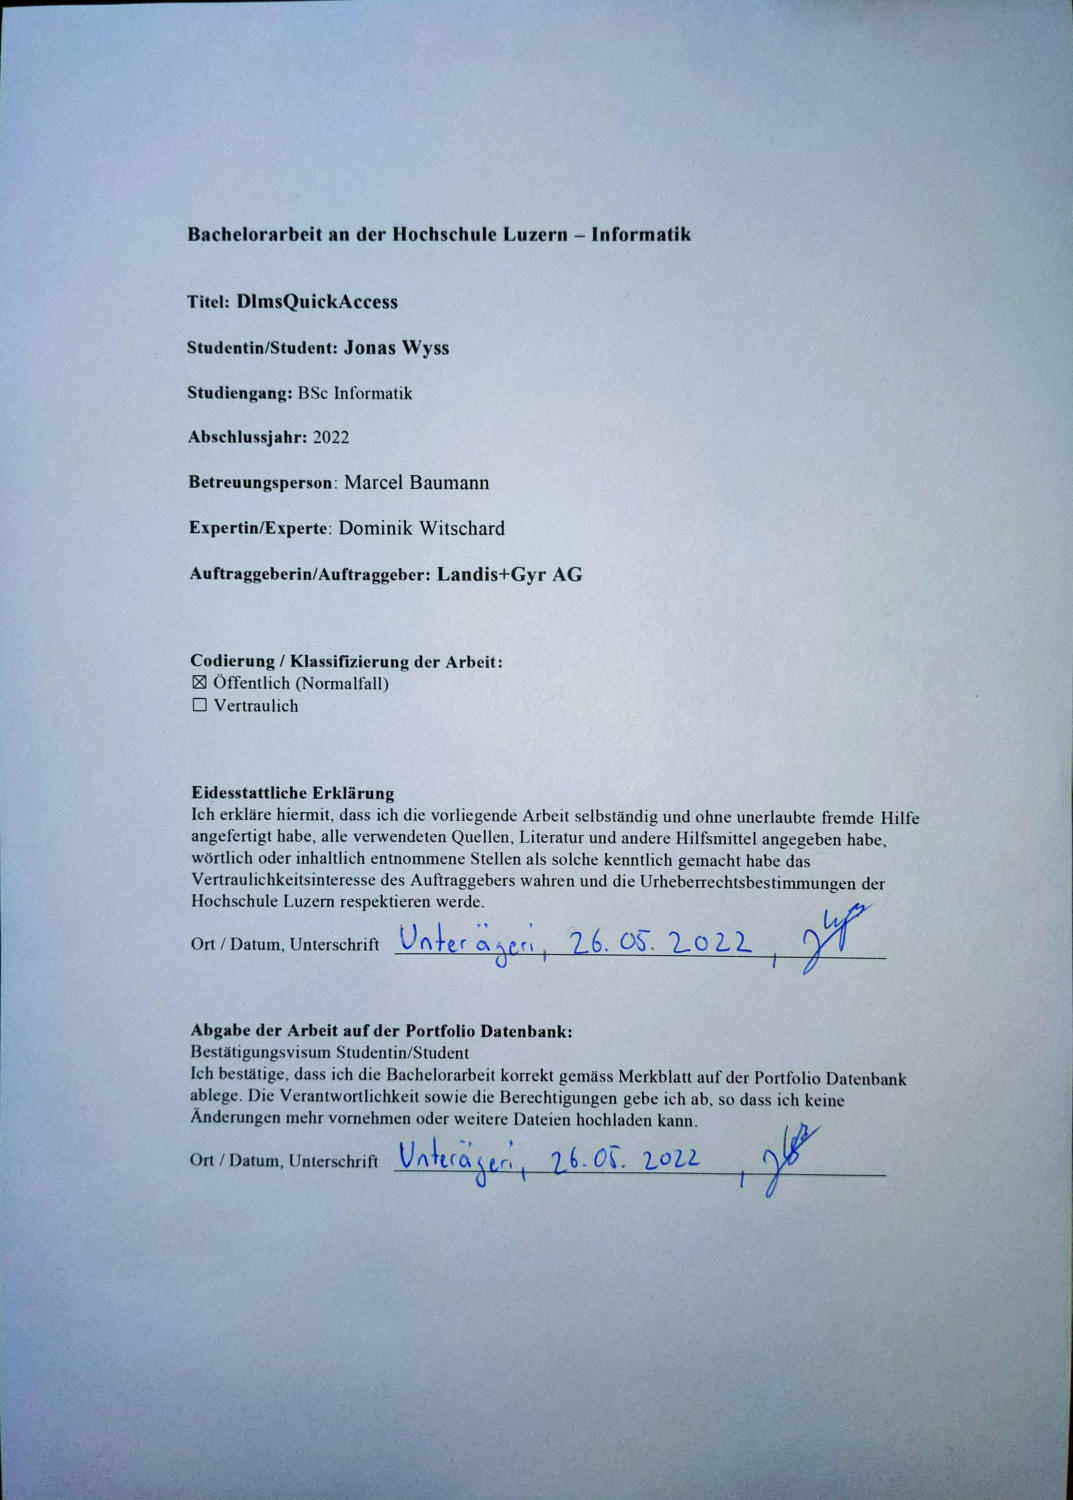
\includepdf[pages=-]{frontbackmatter/bas2}
\section{Verdankungen}

Als erstes möchte ich mich bei meinem Betreuer, Herrn Marcel Baumann bedanken.
Sie haben mich während meiner Arbeit kompetent begleitet, herausgefordert und motiviert.

Vielen Dank an meine Arbeitgeberin, die Landis+Gyr AG.
Während meines Studiums konnte ich das Gelernte in meiner Teilzeitstelle direkt im Beruf anwenden.
In den letzten vier Jahren zeigten meine Kollegen und Vorgesetzten viel Flexibilität und unterstützten mich wo immer möglich.
Ich hoffe, dass ich mit dieser Arbeit einen Teil zurückgeben kann.

Ein besonderer Dank gilt jenen Personen, welche mir bei meiner Arbeit in Form von Tipps, Expertenwissen oder Korrekturlesungen halfen.
%\cleardoublepage\include{frontbackmatter/Dedication}
%\cleardoublepage\include{frontbackmatter/Foreword}
% \cleardoublepage%*******************************************************
% Declaration
%*******************************************************
\refstepcounter{dummy}
\pdfbookmark[0]{Declaration}{declaration}
\chapter*{\condENGLISH{Declaration}{Erklärung}}

\textbf{Codierung / Klassifizierung der Arbeit:}\\
\\
$\square$ \"Offentlich
$\square$ Vertraulich

\paragraph{\textbf{Eidesstattliche Erkl\"arung}}
Ich erkl\"are hiermit, dass ich/wir die vorliegende Arbeit selbst\"andig und ohne unerlaubte fremde Hilfe angefertigt haben, alle verwendeten Quellen, Literatur und andere Hilfsmittel angegeben haben, w\"ortlich oder inhaltlich entnommene Stellen als solche kenntlich gemacht haben, das Vertraulichkeitsinteresse des Auftraggebers wahren und die Urheberrechtsbestimmungen der Hochschule Luzern respektieren werden. \newline \newline
Ort / Datum, Unterschrift	\underline{\hspace*{8cm}} \newline \newline
Ort / Datum, Unterschrift	\underline{\hspace*{8cm}} \newline \newline \newline
\textbf{Ausschliesslich bei Abgabe in gedruckter Form: \\
Eingangsvisum durch das Sekretariat auszuf\"ullen}\newline \newline
Rotkreuz, den	\underline{\hspace*{4cm}}	\hspace*{1cm} Visum:	\underline{\hspace*{4cm}}

\condLOCK{\cleardoublepage%*******************************************************
% Declaration
%*******************************************************
\refstepcounter{dummy}
\pdfbookmark[0]{Blocking Notice}{blocking notice}
\chapter*{\condENGLISH{Blocking notice}{Sperrvermerk}}
\thispagestyle{empty}

Diese Abschlussarbeit darf nur von der Referentin/ dem Referenten, der Korreferentin / dem Korreferenten sowie den vom Prüfungsausschuss dazu beauftragten Hochschulangehörigen eingesehen werden. Sie darf ohne ausdrückliche Zustimmung des Autors
weder vollständig noch auszugsweise vervielfältigt, veröffentlicht oder Dritten zugänglich gemacht werden. Die Durchführung des Kolloquiums bleibt von der Geheimhaltung unberührt. Die Geheimhaltungsverpflichtung erlischt fünf Jahre nach Einreichung automatisch.
}
\cleardoublepage%*******************************************************
% Abstract
%*******************************************************
%\renewcommand{\abstractname}{Abstract}
\begingroup
\let\clearpage\relax
\let\cleardoublepage\relax
\let\cleardoublepage\relax

\cleardoublepage


\pdfbookmark[0]{Abstract}{Abstract}
\chapter*{Abstract}
Die vorliegende Arbeit beschriebt den Entwicklungsprozess einer Software welche von der Landis+Gyr AG in Auftrag gegeben und von einem Bachelor Studenten der Hochschule Luzern erarbeitet wurde.

Eine veraltete Software, welche bei der Entwicklung intelligenter Stromzähler zu Debugging- und Testing-Zwecken eingesetzt wird, wird durch eine Neuentwicklung ersetzt.
Die Nutzer dieser Software werden in Entwicklungsprozess mehrmals mit einbezogen.
Bei der Entwicklung wird speziellen Wert auf Softwarequalität und Usability gelegt.
Der aktuelle Stand der Theorie und der Technik zu diesen und weiteren Themen wird aufgearbeitet.

Des Weiteren werden Ideen, Konzepte und Methoden erklärt, welche für das Projekt relevant sind.
Eine Technologieevaluation gibt Auskunft, wieso C\# und WinUI3 für die Entwicklung eingesetzt wurden.
Das iterative Vorgehen wird detailliert beschrieben.
Nebst Entwicklungs- und Programmierarbeiten gehören dazu auch beispielsweise das Aufsetzten einer Continuous-Integration-Pipeline auf Azure DevOps oder die Qualitätssicherung mittels SonarQube.

Das erstellte Produkt wird anhand der Theorie sowie Rückmeldungen der Nutzer validiert.
Abschliessend wird festgehalten, welche Arbeiten noch offen stehen und wie die Software weiter verbessert werden kann.
\endgroup

\vfill

\cleardoublepage%*******************************************************
% Table of Contents
%*******************************************************
\pagestyle{scrheadings}
\refstepcounter{dummy}
\pdfbookmark[0]{\contentsname}{tableofcontents}
\setcounter{tocdepth}{2} % <-- 2 includes up to subsections in the ToC
\setcounter{secnumdepth}{3} % <-- 3 numbers up to subsubsections
\manualmark
\markboth{\spacedlowsmallcaps{\contentsname}}{\spacedlowsmallcaps{\contentsname}}
\tableofcontents

\cleardoublepage

%\cleardoublepage%*******************************************************
% List of Tables
%*******************************************************
\automark[section]{chapter}
\renewcommand{\chaptermark}[1]{\markboth{\spacedlowsmallcaps{#1}}{\spacedlowsmallcaps{#1}}}
\renewcommand{\sectionmark}[1]{\markright{\thesection\enspace\spacedlowsmallcaps{#1}}}
\refstepcounter{dummy}
\pdfbookmark[0]{\listtablename}{lot}
\listoftables

\cleardoublepage

%\cleardoublepage%*******************************************************
% List of Listings
%*******************************************************      
\automark[section]{chapter}
\renewcommand{\chaptermark}[1]{\markboth{\spacedlowsmallcaps{#1}}{\spacedlowsmallcaps{#1}}}
\renewcommand{\sectionmark}[1]{\markright{\thesection\enspace\spacedlowsmallcaps{#1}}}
\refstepcounter{dummy}
\pdfbookmark[0]{\lstlistlistingname}{lol}
\lstlistoflistings

\cleardoublepage

%*************************************************************************
% Mainmatter
%*************************************************************************
\cleardoublepage
\pagestyle{scrheadings}
\pagenumbering{arabic}
% Alwas use \cleardoublepage before \part{...}.
\cleardoublepage
% \part{Thesis}\label{pt:thesis}
\chapter{Problem, Fragestellung, Vision}

% Aus Aufbau_Bericht.pdf
% Welche Ziele, Fragestellungen werden mit dem Projekt verfolgt? Die Bedeutung, Auswirkung und
% Relevanz dieses Projektes für die unterschiedlichen Beteiligten soll aufgeführt werden.
% Typischerweise wird hier ein Verweis auf die Aufgabenstellung im Anhang gemacht.
\chapter{Stand der Technik}

Das folgende Kapitel gibt einen Einblick in den Stand der Technik und Hingergrundinformationen
für diese Arbeit.

\section{Einführung}

TODO: Jonas, Stand der stromzähler Technik.

Ein Stromzähler \cite{wikipedia:meter} misst den Stromverbrauch eines Haushaltes über eine
Zeitspanne. Diese Daten können sowohl für den Endverbraucher als auch für Kraftwerke
und Verteiler interessant sein. Beispielsweise können \ac{THD} \cite{siemens:disw_2021}
Werte eine Aussage über den Zustand eines Generators in einem Kraftwerk machen. \cite{thd-generators}

Moderne Stromzähler verfügen über zu wenig Rechenleistung um die Daten lokal
aufbereiten zu können. \cite{dc450-technical-data}
Aus diesem Grund sollen die Daten via \ac{MQTT} \footnote{https://mqtt.org/} Protokoll
an einen Server zur Weiterverarbeitung gesendet werden.

\ac{MQTT} eignet sich vor allem für \ac{IoT} Geräte mit geringer Leistungsfähigkeit
und wurde vom Auftraggeber bereits so vorgegeben, da Sie von verschiedenen
Stromzählern bereits unterstützt wird.

\section{Hosting und Deployment}

Zu beginn des Projektes war die Idee, das Projekt in der Google Cloud zu hosten.
Da jedoch die Infrastruktur auf Seiten des Auftraggebers noch nicht dazu bereit
war, konnte dies nicht umgesetzt werden. Stadtdessen soll eine möglichst
generische lösung, welche vielleicht später auf einen Kubernetes\footnote{https://kubernetes.io/}
Cluseter deployen zu können. Damit ein Produkt reproduzierbar
deployt werden kann, werden heutzutage Container verwendet. \cite{what-is-a-container}

Das wohl bekannteste und weit verbreitetste Container Framework
ist Docker\footnote{https://www.docker.com/}. Docker hat jedoch einige Nachteile.
So ist Docker beispielsweise per default nicht rootless.\cite{docker:rootless}
Das bedeutet, dass ein in einem Container gestarteter Prozess als root user
auch auf dem Host system unter der gleichen Benutzer läuft. Wenn jetzt also
der Prozess aus der Containerisolation ausbricht\footnote{Dies kann beispielsweise durcheine Sicherheitslücke passieren}
ist er auch auf dem Hostsystem root.\cite{so_2020}
Zudem ist Docker an einen Damon gebunden, der im Hintergrund läuft.
Dadurch werden alle Container neu gestartet wenn der Daemon neu gestartet werden muss.\cite{docker:daemon}
Aus diesen gründen setzen viele Projekte podman\footnote{https://docs.podman.io/en/latest/}
als Container Engine ein. Podman ist rootless by default und erlaubt Daemonless Container.
Zudem können multicontainer Projekte einfach mit Kubernetes Config files
erstellt werden.\cite{redhat:podman-pods}



\chapter{Ideen und Konzepte}
TODO einleitung

% Hier geht es um die Fragestellung, wie Sie die formulierten Ziele der Arbeit erreichen wollen.
% Sie halten z.B. erste, grobe Ideen, skizzenhafte Lösungsansätze fest. Gibt es mehrere Wege, Ansätze
% um dieses Ziel zu erreichen, begründen Sie hier, warum Sie einen bestimmten Weg einschlagen.
% Beispiel für ein Softwareprojekt: Erste Gedanken über eine grobe Systemarchitektur. Ist z.B. eine
% Microservice-Architektur angebracht? Welche Alternativen bestehen, wo gibt es Problempunkte? Die
% Umsetzung, die Beurteilung der Machbarkeit und die detaillierte Beschreibung der umgesetzten
% Architektur sind dann Teil der Realisierung.
% Abgrenzung zu Kapitel 5:
% - Besteht ein wesentliches Projektziel darin, für Ihre Kunden z.B. ein Security-Konzept, ein
% Kommunikations-Konzeptes, ein IT-Fachkonzept oder ein anderes Fach-Konzept zu erstellen, dann
% wird die Entwicklung dieser (fachlichen) Konzepte unter «Realisierung» beschrieben (sie sind ja der
% eigentliche Kern Ihrer Arbeit).
% - Besteht z.B. ein wesentliches Ziel der Arbeit darin, eine passende Software-Architektur zu
% evaluieren, dann gehören die entsprechenden Beschreibungen ins Kapitel 5.


% \section{Konfiguration} \label{idea_config} %todo delete
% \subsection{Motivation}
% Bei der Landis+Gyr werden verschiedenen Stromzählermodelle entwickelt. Der DlmsQuickAccess soll mit möglichst allen kommunizieren können.
% Wie bereits in XY TODO erwähnt, wird für die Kommunikation Code der ATS verwendet.
% Damit dieser richtig funktionieren kann, werden folgende zwei Dateien benötigt:
% - AddressList
% - DLMS.xml
% Für die Auflistung aller Objekte eines Zählers wird zusätzlich ein ObjectModel als XML Datei benötigt.
% Diese drei Dateien unterscheiden sich von Produkt zu Produkt. Ebenfalls muss berücksichtigt werden, dass sich die Informationen in diesen Dateien jederzeit ändern können.
% Insbesondere beim ObjectModel ist dies regelmässig der Fall.

% Diese Konfigurationen sollen somit von den Produktteams verwaltet und versioniert werden können.

% \subsection{Lösungsidee}
% Eine Konfigurationsdatei in welcher die zuvor erwähnten Dateien definiert sind. Die soll im YAML format geschrieben sein, was das Bearbeiten vereinfacht.
% Jedes Produktteam kann diese Konfigurationsdatei im Repository des Produktquellcodes ablegen und versionieren.

% TODO
% damit sich der DlmsQuickAccess beim Betriebssystem so registrieren kann, dass 
% Diese Konfiurationsdateien sollen die Endung \".dlmsquickaccess\" tragen, 

% Um das Wechseln zwischen Produkten zu vereinfachen, soll sich der DlmsQuickAccess zuvor verwendete Konfigurationen merken, so dass der Benutzer diese auswählen kann.


% TODO ufschribe, was passiert bim erste start und bi doppelclick.


\section{Aufbau Benutzerschnittstelle}\label{aufbauUI}
Die Benutzerschnittstelle soll in zwei Bereiche aufgeteilt werde.
\begin{figure}[H]
   \centering
   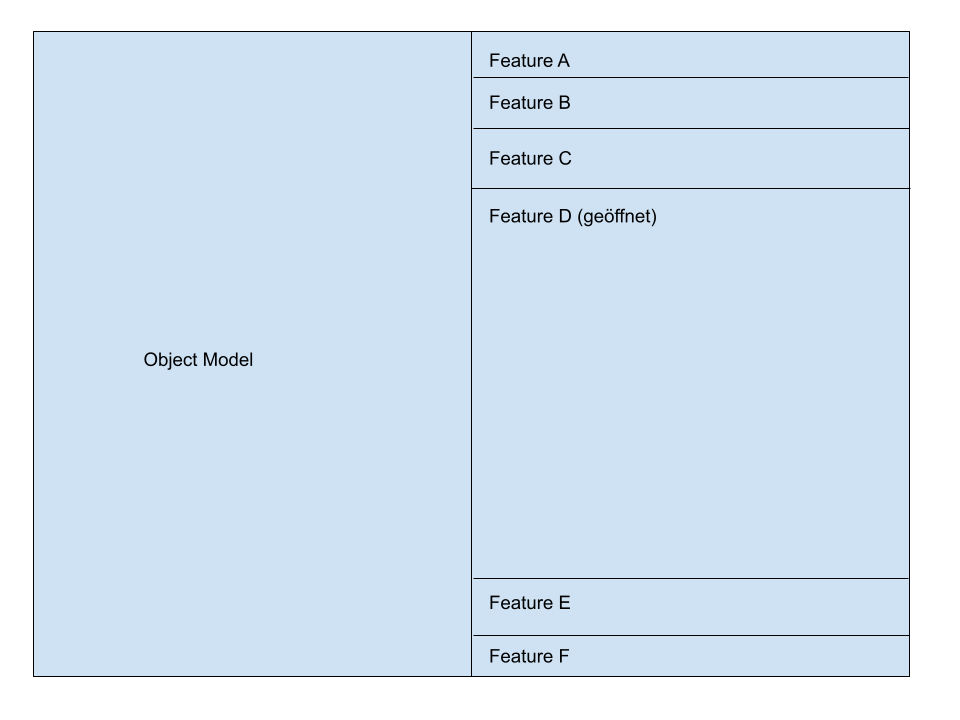
\includegraphics[width=1.0\textwidth]{gfx/App strucutre sketch.png}
   \caption{
      Sketch des Aufbau der Benutzeroberfläche
      }
      \label{fig:uisketch}
   \end{figure}
Der erste Bereich soll Object Model beinhalten.
Im folgenden Abschnitt wird darauf detailliert eingegangen.
Dieser Bereich soll alle Grundfunktionen der Applikation abdecken.
Also jene, welche bei der zu ersetzenden Applikation, dem \textit{DMT2} vorhanden sind.
Der zweite Bereich soll Platz für die erweiterten Funktionen bieten.
Die Idee ist, dass diese vertikal übereinander aufgelistet sind.
Möchte der Nutzer eine Funktion verwenden, so kann er diese anklicken und entsprechenden Controls erscheinen in der Liste.
In Abbildung \ref{fig:uisketch} ist gezeigt, wie die beiden Bereiche horizontal nebeneinander angezeigt werden sollen.
Auf der rechten Seite ist zu erkennen, wie die verschiedenen Features übereinander aufgelistet werden sollen.
\textit{Feature D} nimmt dabei mehr Platz ein als die anderen.
Damit wird dargestellt, dass dieses von Nutzer angewählt und geöffnet wurde.
Eine dieser Funktionen sind die Favoriten.
Wie deren Benutzerschnittstelle aussehen soll, ist im Abschnitt \ref{uifavorites} aufgeführt.

\subsection{Object Model}
Der \textit{Quick Access} des \ac{DMT2} besteht aus vier Teilen.
In Abbildung \ref{fig:dmt2QuickAccess} ist dies dargestellt.
Oben links sind alle Objekte angezeigt.
Rechts daneben werden die Attribute und Methoden des aktuell aktiven Objekts angezeigt.
Fürs Lesen und Schreiben werden in den unteren beiden Teilen des Fensters jeweils der Request und die Response in einer als \text{XML} Text dargestellt.

\begin{figure}
   \centering
   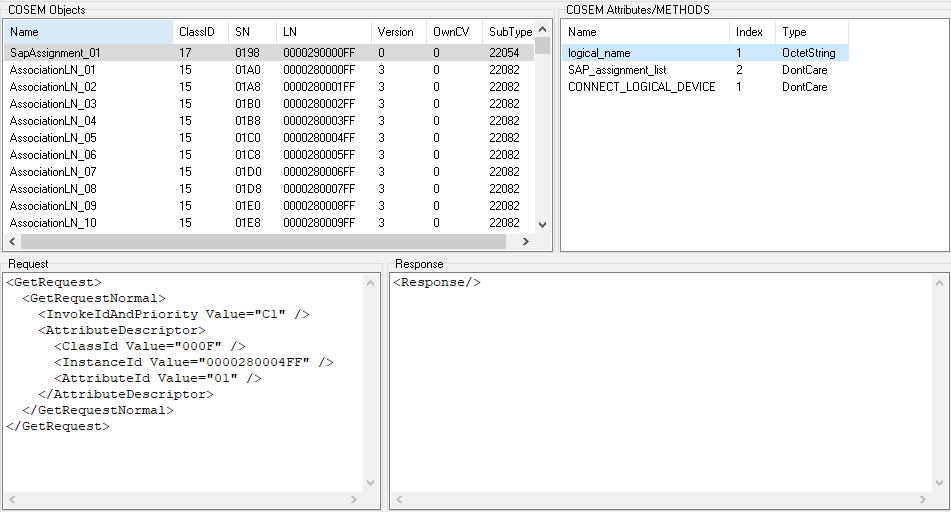
\includegraphics[width=1.0\textwidth]{gfx/UI_DMT2.png}
   \caption{
      Quick Access Fenster des \ac{DMT2}
      }
      \label{fig:dmt2QuickAccess}
\end{figure}
In der neuen Anwendungen sollen diese viert Teile in einer einzelnen Komponente kombiniert dargestellt werden.
Wie dies aussehen kann, ist in Abbildung \ref{fig:objectModelUIsktech} gezeigt.
Die Objekte, beispielsweise \textit{Profile 1}, werden untereinander aufgelistete.
Wird ein Objekt angeklick, soll vergrössert sich dieses und die Attribute und Methoden werden ersichtlich.
Wird ein Attribute gelesen, so soll der Wert in einem Textfeld neben dem Attribut dargestellt werden.
Das bietet den Vorteil, dass die Werte mehrere ausgelesener Attribute gleichzeitig angeschaut werden können. 
Dies ist beim \textit{Quick Access} nicht möglich, da der Bereich mit der Response bei jedem Auslesen überschrieben wird.
Die Textfelder, welche für das Anzeigen der gelesenen Werte verwendet werden, sollen jeweils auch für das Schreiben von Werten verwendet werden.

\begin{figure}
   \centering
   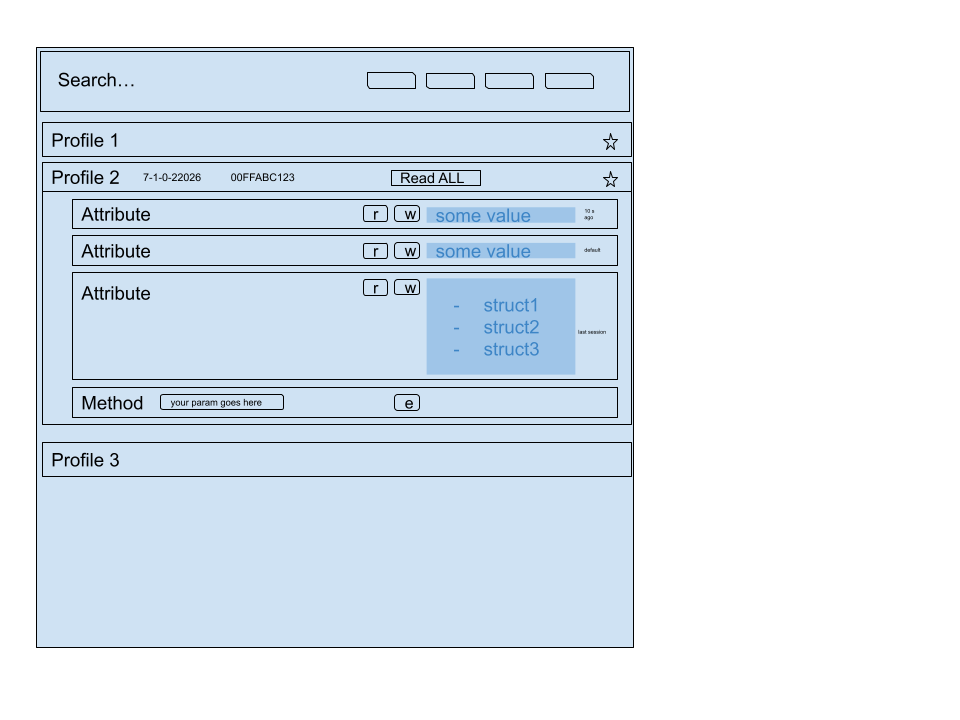
\includegraphics[width=1.0\textwidth]{gfx/Object Explorer Sketch.png}
   \caption{
      Sketch der Object Model Komponente
      }
      \label{fig:objectModelUIsktech}
\end{figure}


\subsection{Suchen und filtern}\label{searchandfilterUiSktech}
Im Sketch zum Object Model (Abbildung \ref{fig:objectModelUIsktech}) ist der Bereich oberhalb der Objekte für die Such- und Filterkomponente vorgesehen.
Eine Idee zur Umsetzung dieser ist in Abbildung \ref{fig:searchFilterSketch}.
Um die Objekte nach ClassId zu filtern, können die Textfelder im oberen Bereich des Sketchs verwendet werden.
Das Textfeld im unteren Bereich ist für die textbasierte suche gedacht.
Ein Schalter in der Mitte soll dazu da sein, dass bei der Textsuche zwischen Objekten und Attributen rsp. Methoden gewechselt werden kan.
Der \textit{Find} Knopf soll die Parameter anwenden, mit dem \textit{Reset} Knopf sollen diese zurückgesetzt werden.

\begin{figure}
   \centering
   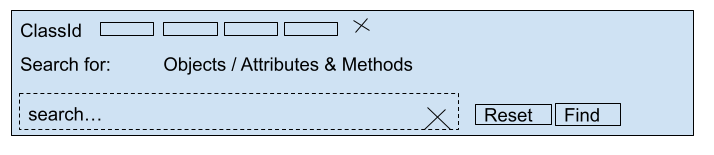
\includegraphics[width=1.0\textwidth]{gfx/Search _ Filter sketch.png}
   \caption{
      Sketch der Komponente fürs Suchen und Filtern des Object Models
      }
      \label{fig:searchFilterSketch}
\end{figure}

\subsection{Favoriten}\label{uifavorites}
In einem vorherigen Abschnitt wurde erklärt, dass auf die rechte Hälfte der Benutzerschnittstelle Platz für unterschiedliche Features haben soll.
Dort sollen auch die Favoriten aufgelistete werden.
Diese sollen in zwei Bereichen dargestellt werden und nehmen somit auch zwei Plätze in der Features Liste ein.
Einer für favorisierte Objekte und einer für favorisierte Attribute und Methoden.
In Abbildung \ref{fig:favoritesSketch} ist ersichtlich, wie Attribute und Methoden gruppiert dargestellt werden sollen.

\begin{figure}
   \centering
   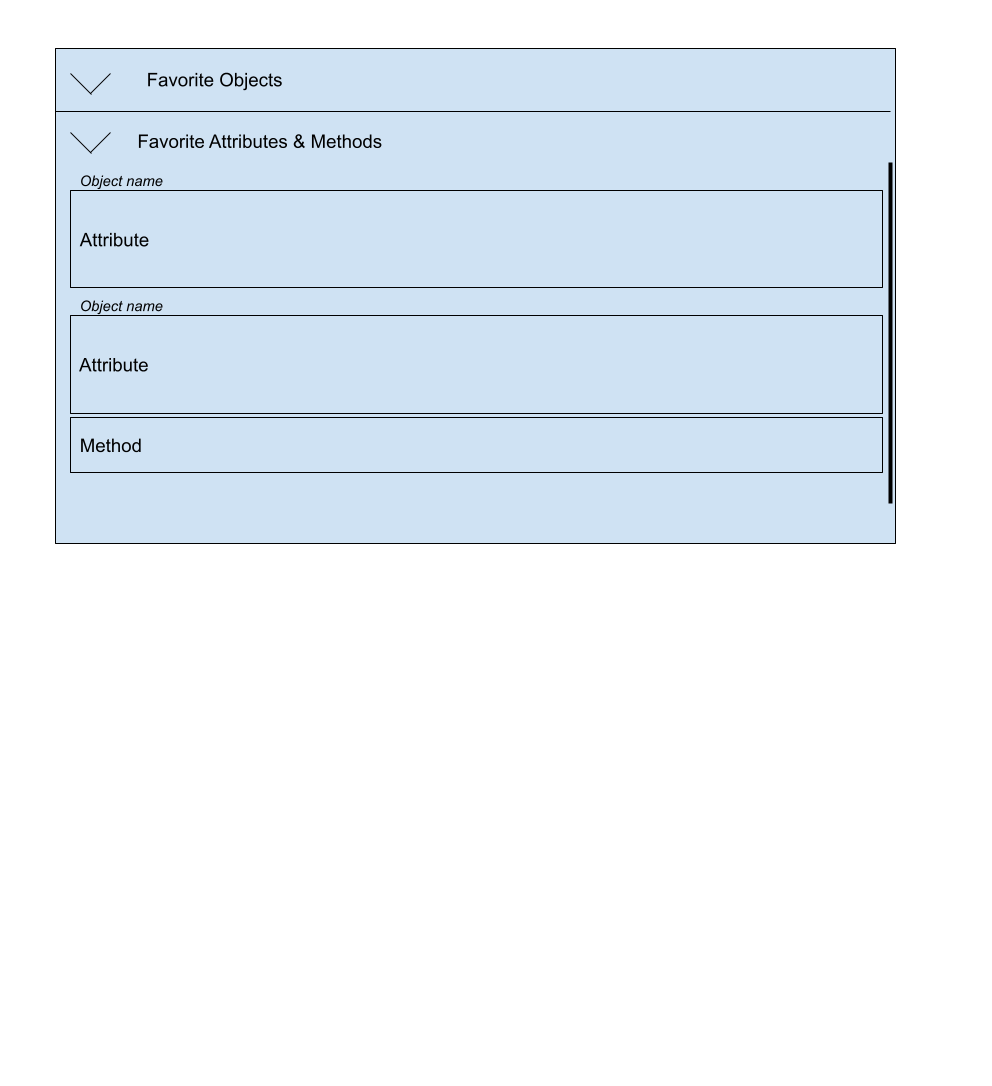
\includegraphics[width=1.0\textwidth]{gfx/Favorites Sketch.png}
   \caption{
      Sketch der Favoriten Komponente
      }
      \label{fig:favoritesSketch}
\end{figure}

\pagebreak
\section{Testkonzept}
Um sicherstellen, dass die Applikation und deren Komponenten richtig funktionieren, wurden verschieden Arten von Tests eingesetzt.
Die unterscheiden sich primär im Umfang des Getesteten. 
In den folgenden Abschnitten werden sie detailliert beschrieben und verglichen.

\subsection{Unittests}
Unittests werden so eingesetzt, dass sie die Funktionalität einer einzelnen Klasse testen.
Abhängigkeiten zu anderen Klassen sollen jeweils durch Mocks ersetzt werden.
Die Tests werden jeweils parallel zum getesteten Code geschrieben.
Mehr dazu im Abschnitt \ref{tdd} Test Driven Development.
Um sicherzustellen, dass zuvor implementierte Funktionen nicht durch neue Änderungen nicht zerstört werden, werden alle Unittest regelmässig und automatisiert ausgeführt.
Dies wurde mit der CI/CD Pipeline realisiert. Diese ist im Abschnitt TODO detailliert beschrieben.

\subsection{Modultests}
Bei den Modultests wird das Zusammenspiel mehrere Klassen getestet, welche gemeinsam ein Modul bilden.
Dabei soll nur das öffentliche Interface des Moduls verwendet werden.
Abhängigkeit, welche nicht Teil dieses Moduls sind, werden wie bei den Unittests durch Mocks oder Fakes ersetzt.
Im Gegensatz zu den Unittests ist der Zeitpunkt für das Schreiben der Modultests nicht definiert.
Sie sollen so eingesetzt werden, wie sie für den Entwicklungsprozess hilfreich sind.

Beispiel: Mittels Refactoring soll das interne Design eines bestehenden Moduls verbessert werden.
Um sicherzustellen, dass das Modul nach dem Refactoring noch korrekt funktioniert, werden zuvor Modultests geschrieben, welche die öffentliche Schnittstelle des Moduls testet.
Da sich diese beim Refactoring nicht verändert, können die Modultests auch noch nach dem Refactoring ausgeführt werden.
Unittests, welche interne Klassen getestet haben sind womöglich nicht mehr brauchbar, da sich die internen Schnittstellen bei Refactoring stark verändert haben.

Im Bezug auf die regelmässige und automatisierte Ausführung sollen sich Modultests nicht von Unittests unterscheiden.


\subsection{Integrationstests}\label{Integrationstests}
Integrationstests sind im dazu da, die Funktionalität von Komponenten sowie das Zusammenspiel dieser mit anderen zu Testen \parencite{winter2012integrationstest}.
Im Gegensatz zu Unit- und Modultests wird auf den Einsatz von Mocks oder Fakes verzichtet um ein möglichst realitätsnahen Testaufbau zu erreichen.
Da die Kommunikation mit Stromzähler für die zu testende Applikation zentral ist, wird für das Ausführen der Integrationstests ein angeschlossener Stromzähler benötigt.
Im Rahmen dieses Projekts war es nicht mögliche einen Testagent mit angeschlossenem Zähler bereit zu stellen.
Deshalb wurden die Integrationstests ausschliesslich lokal auf dem Rechner des Entwicklers ausgeführt.


\section{Model-View-ViewModel}\label{mvvm}
\ac{MVVM} ist ein Entwurfsmuster welches 2005 von Microsoft vorgestellt wurde.
Sein Ziel ist es, das Daten, Logik und Views einer Anwendung unabhängig von einander entwickelt und getestet werden können.
Es besteht aus folgenden Sichten:
\begin{itemize}
   \item Model: Das Domänen Model der Applikation
   \item View: XAML Komponenten, welche die visuellen Aspekte der Applikation definieren
   \item ViewModel: Klassen bestehend aus Properties und Commands, welche von den Views verwendet verden
\end{itemize}

% TODO Image source : https://www.dev-insider.de/was-bedeutet-mvvm-a-1103448/
\begin{figure}[H]
   \centering
   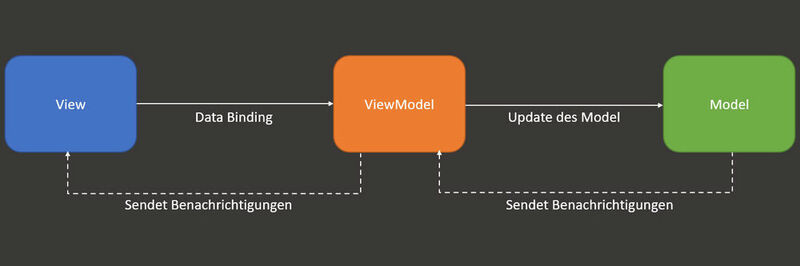
\includegraphics[width=1.0\textwidth]{gfx/mvvm.jpg}
   \caption{
      Das Model-View-ViewModel Entwurfsmuster
   }
   \label{fig:mvvm}
\end{figure}
Die ViewModels sind dabei der wichtigste Teil, da sie den Zustand der Applikation abbilden.
Sie sammeln die für die Views benötigten Daten zusammen und stellen sie als Properties bereit.
Mittels DataBinding referenzieren die Views diese Properties, ohne dabei das konkrete ViewModel kennen zu müssen \parencite{vermeir2022desktop}.
Wie \ac{MVVM} für diese Arbeit umgesetzt werden kann, ist im folgenden Abschnitt beschrieben.




\section{Architektur}
% TODO, evtl verschieben zu Realisierung und hier nur die grundlegenden Idee aufzeigen. Wie MVVM angewendet wurde
Der Quellcode der Anwendung ist in mehrere C\# Projekte aufgeteilt.

Dies soll die Wiederverwendbarkeit der Komponenten sicherstellen.
Wenn in Zukunft eine Komponente wie bspw. die Kommunikation ausgetauscht werden soll, so müssen nur in einem spezifischen Teil des Codes Änderungen vorgenommen werden.

\begin{figure}[H]
   \centering
   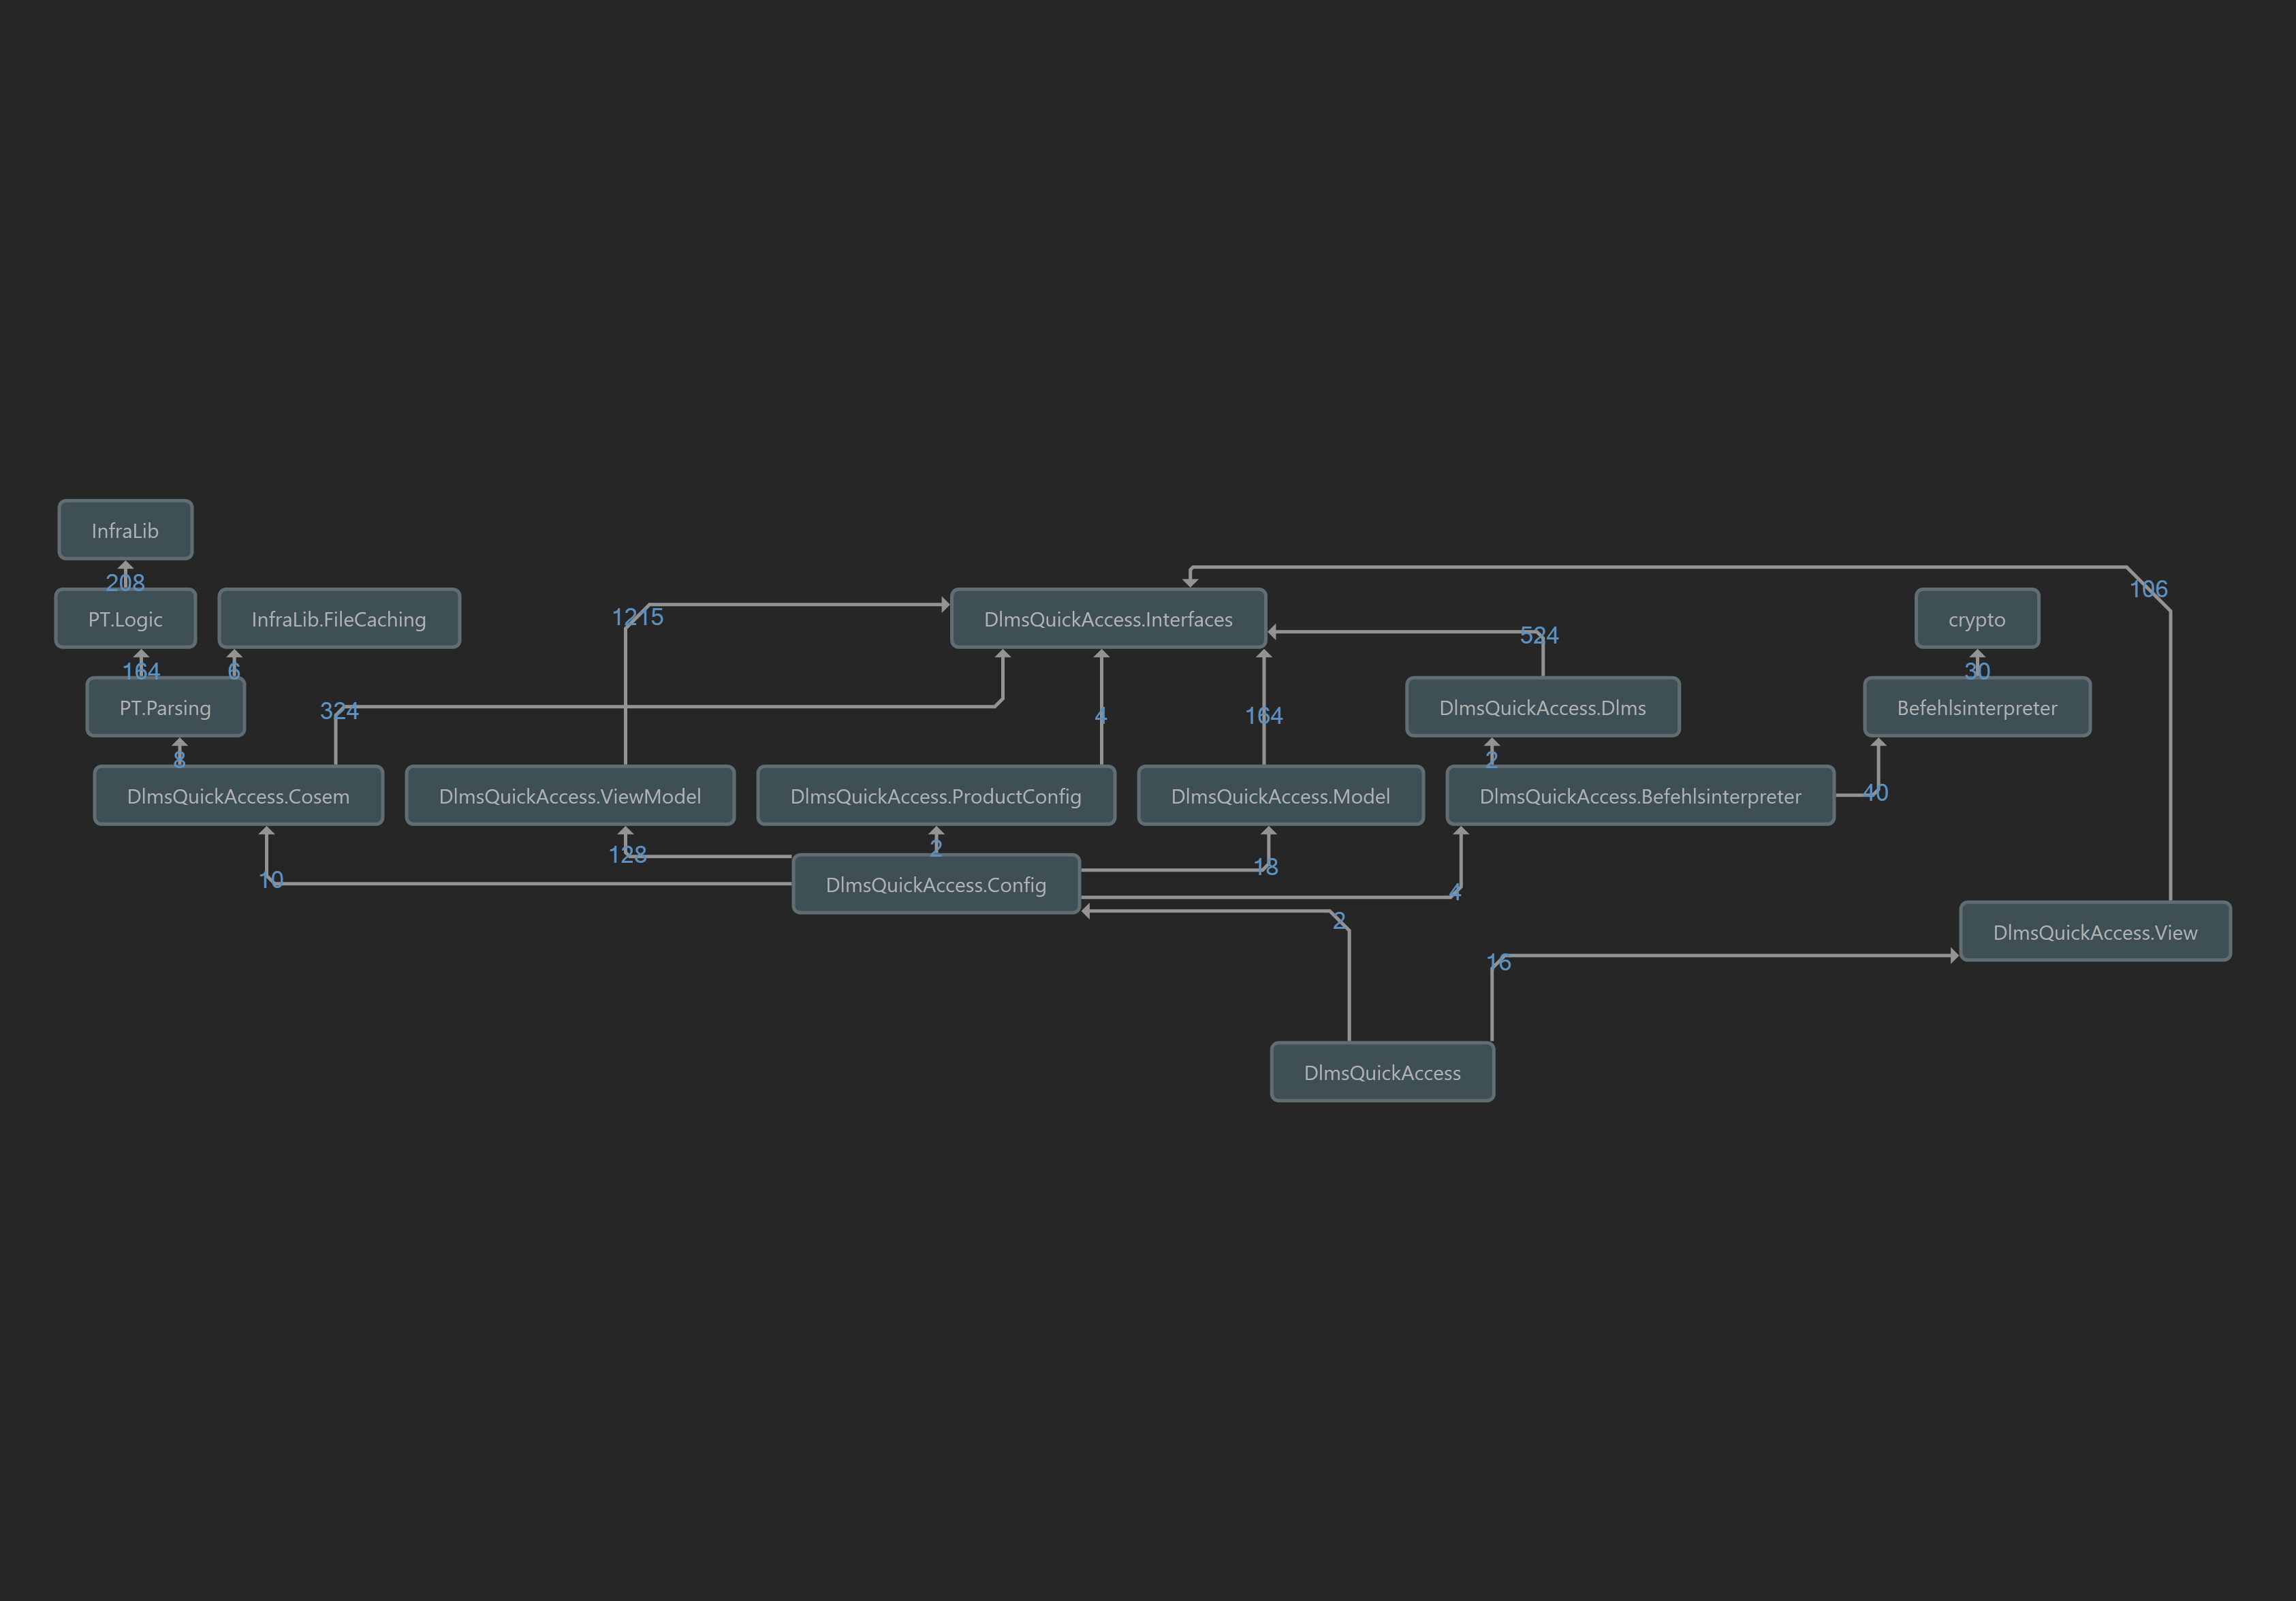
\includegraphics[width=1.0\textwidth]{gfx/Architecture view for DlmsQuickAccess.png}
   \caption{
      Abhänigkeiten der Projekte
   }
   \label{fig:projectDependencies}
\end{figure}

In der Abbildung \ref{fig:projectDependencies} sind alle\footnote{Die Testprojekte wurde einfachheitshalber weggelassen.} Projekte und deren Abhängigkeit aufgezeigt.
Diese werden in den folgenden Abschnitten näher beschrieben.

\subsection{DlmsQuickAccess}
Dieses Projekt ist der Einstiegspunk der Anwendung.
Die Klasse \textit{App} lässt sich mit der \texttt{main()} Method vergleichen, welchen den meisten C basierten Sprachen als erstes ausgeführt, wenn ein Programm gestartet wird.
Diese lädt \textit{Windows} und \textit{Controls} aus dem DlmsQuickAccess.View Projekt und zeigt diese dem Nutzer an.



\subsection{DlmsQuickAccess.View}
Sämtliche Komponenten der Benutzerschnittstelle, also \textit{Windows} und \textit{Controls}, sind in diesem Projekt definiert. 
Nebst der Abhängigkeit zum Framework WinUI3, welches für die Darstellung der Element der Benutzerschnittstelle benötigt wird, gibt es nur eine einzige Abhängigkeit, jene zu DlmsQuickAccess.Interfaces.
Diese ist dazu da, dass die Controls die Interfaces der ViewModels kennen, auf welche sie binden.
Das Zusammenspiel von View und ViewModel ist im Abschnitt \ref{mvvm} beschrieben.
Währen diese Interfaces im selben Projekt wie die Controls definiert, so hätten die Implementationen der ViewModels eine Abhängigkeit auf DlmsQuickAccess.View.
Um eine solche Koppelung zu vermeiden, wurden die Interfaces in ein eigenes Projekt ausgelagert.


\subsection{DlmsQuickAccess.ViewModel}
Die zuvor erwähnten ViewModel Interfaces sind in diesem Projekt implementiert.
Nebst den eigentlichen ViewModel Klassen enthält das Projekt mehrere Factory Klassen, welche für die Instanziierung der ViewModel Klassen zuständig sind.
Hier wurde das Factory Method Erstellungsmuster angewendet \parencite{designPatterns}.
In Abbildung \ref{fig:filterViewModel} ist die \textit{FilterViewModelFactory} Klasse zur Erstellung des \textit{FilterViewModel} aufgezeigt.
\begin{figure}[H]
   \centering
   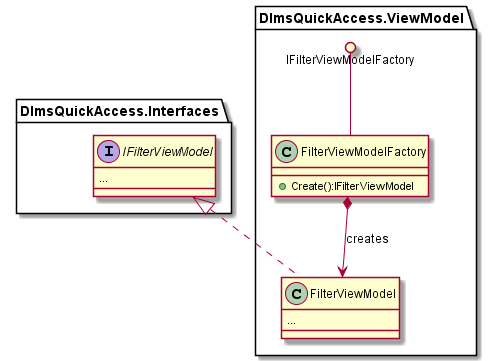
\includegraphics[width=0.7\textwidth]{gfx/Filter ViewModel.png}
   \caption{
      Unvollständiges Klassendiagramm zum FilterViewModel und FilterViewModelFactory
      }
      \label{fig:filterViewModel}
\end{figure}

Dieses Design vereinfacht das Testen der Instanziierungen.
Ein weitere Vorteil ist, dass eine Factory eine andere Factory mittels Assoziation verwenden kann, deren konkrete Implementation jedoch nicht kennen muss.
In Abbildung \ref{fig:vmfactories} ist ganz oben die \textit{MainWindowViewModelFactory} Klasse abgebildet, welche für die Erstellung des \textit{MainWindowViewModel} zuständig ist.
Dieses ViewModel beinhaltete alle anderen ViewModels welche für die verschiedenen Bereiche der Applikation benötigt werden.
Um diese zu erstellen verwendete \textit{MainWindowViewModelFactory} Instanzen der \textit{IObjectModelViewModelFactory} und \textit{IFavoritesViewModelFactory} welche selbst weitere Factories verwenden.
Das bringt den Vorteil, dass die einzelnen Factory Klassen nicht aneinander gekoppelt sind.
Sie werden erst bei ihrer Instanziierung mittels Dependency Injection miteinander verbunden.
Diese ist Teils des Projekts DlmsQuickAccess.Config (\ref{dqa:config}).
   
\begin{figure}[H]
   \centering
   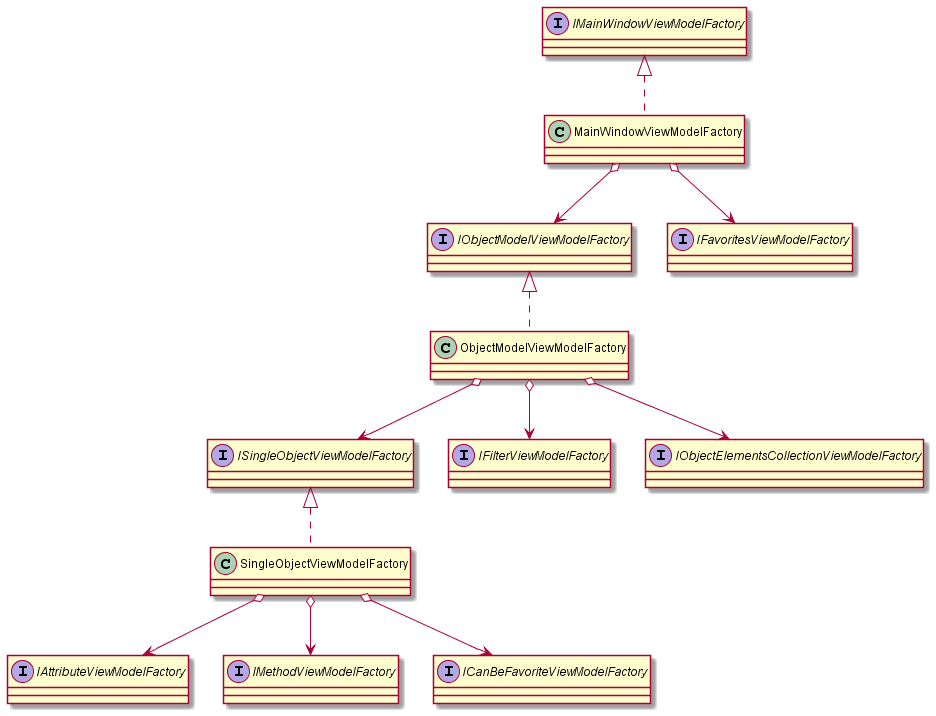
\includegraphics[width=1.0\textwidth]{gfx/vmfactories.png}
   \caption{
      Unvollständiges Klassendiagramm zu den verschiedenen ViewModel Factories.
      }
   \label{fig:vmfactories}
\end{figure}

\subsection{DlmsQuickAccess.Model}


\subsection{DlmsQuickAccess.Config}\label{dqa:config}

\subsection{DlmsQuickAccess.Interfaces}

\subsection{DlmsQuickAccess.ProductConfig}
External dependency to yamllib


\subsection{DlmsQuickAccess.Dlms}
evtl widerverwendbar

\subsection{DlmsQuickAccess.Cosem}
evtl widerverwendbar
infralib etc.

\subsection{DlmsQuickAccess.Befehlsinterpreter}
isolation des Befehlsinterpreter


\chapter{Methoden}

% Aus Aufbau_Bericht.pdf
% Hier halten Sie fest und begründen, welches Vorgehensmodell Sie für Ihr Projekt wählen. Sie
% verweisen allenfalls auf die daraus entstandenen, konkreten Terminpläne mit Meilensteinen, welche
% z.B. unter Realisierung (Kapitel 5) oder im Anhang versorgt sind.

% Bei Engineering-Projekten halten Sie weitere einzusetzende fachliche Methoden oder Techniken fest.
% Bei einem Softwareprojekt können dies z.B. der geplante Einsatz einer Anforderungsanalyse, der
% Einsatz von Review-Techniken (Architektur-Reviews) oder bekannter Programmiertechniken sein.


% TODO evtl einleitung schreiben


\section{Vorgehensmodell}\label{vorgehen}
In der Aufgabenstellung (Anhang \ref{anhang:aufgabenstellung}) wurde verlangt, das der Scrum Prozess, so wie er bei der Landis+Gyr gelebt wird, als Vorgehensmodell verwendet werden soll.
Diverse Eigenschaften und Abläufe dieses Prozesses konnten direkt für diese Arbeit übernommen und angewandt werden.
Da an dieser Arbeit nur ein Entwickler arbeitet und auch die Anzahl Stakeholders kleiner ist, wurde mehrere Dinge angepasst.
Die folgenden Abschnitte geben einen Überblick über den Prozess, wo sich dieser von jeden der Landis+Gyr unterscheidet und wieso diese Anpassungen vorgenommen wurden.

\subsection{Sprints}
Das Projekt besteht aus mehreren aufeinanderfolgenden Sprints.
Jeder Sprint dauert zwei Wochen.
Wären eines Sprints wird an jenen User Stories gearbeitete, welche für diesen Sprint eingeplant sind.
Die Entwickler geben zu Beginn des Sprints das Commitment ab, dass sie die geplanten Stories im Sprint abschliessen werden.
Um weder zu viele Stories noch zu wenige in einem Sprint zu planen, werden bei der Landis+Gyr jeder Story einen Wert gegeben.
Dieser Wert, welche Story Points genannt wird, wird von den Entwicklern geschätzt und beziffert den erwarteten Aufwand.
Auf Story Points wurde bei dieser Arbeit verzichtet, da sie für den Einzelentwickler keinen Mehrwert bieten.

Während die Dauer aller Sprints genau gleich ist variiert die Zeit, welche der Entwickler für Entwicklungsarbeiten aufwenden kann von Sprint zu Sprint stark.

\subsubsection{User Story}\label{userstory}
Der Scrum Prozess der Landis+Gyr kennt viele unterschiedliche Work Items wie z.B. Epics, Requirements oder Features.
In Abbildung \ref{fig:workitems} sind sie alle dargestellt.
\begin{figure}[H]
   \centering
   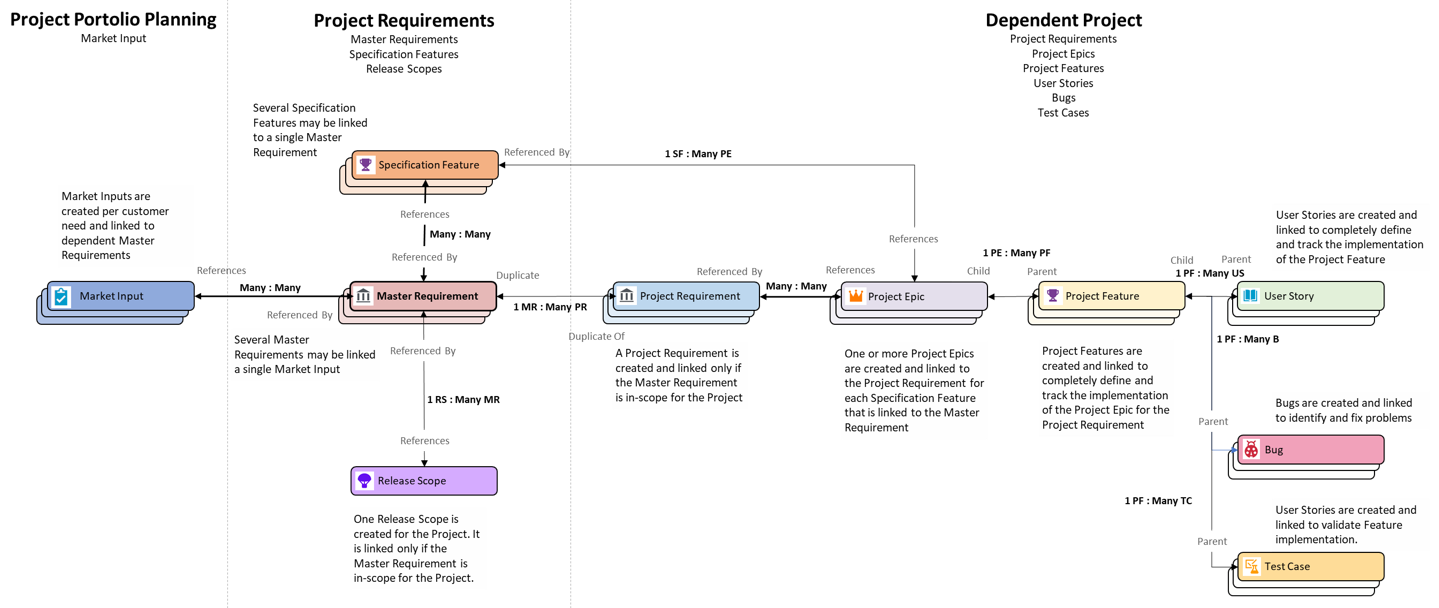
\includegraphics[width=1.0\textwidth]{gfx/WorkItemRelationsship.png}
   \caption{
      Übersicht über die verschiedenen Work Items im Scrum Prozess der Landis+Gyr
      }
      \label{fig:workitems}
\end{figure}
Um möglichst wenig Zeit mit administrativen Aufgaben zu verbrauchen wurde für diese Arbeit nur User Stories eingesetzt.
Eine User Story beschreibt jeweils ein Arbeitspaket welches während eines Sprints vollständig bearbeitet werden kann.
Sie enthält eine Sammlung von Akzeptanzkriterien, welche durch die Bearbeitung der Story erfüllt werden müssen.
Damit eine Story als fertig gilt, muss die Definition of Done erreicht werden. Diese wird im folgenden Abschnitt erläutert.

%todo task?

\subsubsection{Definition of Done}
Für diese Arbeit besteht diese aus folgenden Punkten:
\begin{itemize}
   \item Alle Akzeptanzkriterien sind erfüllt.
   \item Unittests wurden implementiert oder angepasst, decken mindestens 80\% des Codes ab und laufen erfolgreich durch.
   \item Der Code entspricht dem Coding Standard, siehe \ref{codingStandard}.
\end{itemize}

Bei der Landis+Gyr gehört zur Definition of Done zusätzlich noch, dass der Code von mindestens zwei weiteren Entwicklern gegengelesen wurde.
Dies ist bei diesem Projekt leider nicht möglich.


\subsection{Meetings}
Zum Scrum Prozess gehören diverse Meetings, welche regelmässig stattfinden.
So wir ein Sprint jeweils im Voraus während des \textit{Sprint Planning} geplant.
Während des Sprints findet im \textit{Daily Meeting} ein täglicher Austausch zwischen allen Entwicklern statt.
Im \textit{Sprint Review} werden nach einem Sprint die erarbeiteten Stories präsentiert.
Die \textit{Retrospektive}, welche ebenfalls nach jedem Sprint stattfindet, regt die Entwickler dazu an, die eigene Arbeitsprozesse zu reflektieren und diese womöglich zu verbessern.

Alle diese Meetings werden für diese Arbeit weggelassen.
Die Planung des neuen Sprints wird jeweils ad hoc erledigt und Änderungen am Arbeitsprozess sofort umgesetzt.
Während des Projekts finden mehrere Meetings mit der Betreuungsperson dieser Arbeit statt.
Dort werden jeweils die gemachten Fortschritte und erledigten Arbeiten präsentiert.
Somit lassen sich diese teilweise mit dem \textit{Sprint Review} vergleichen.
Sie sind zeitlich jedoch nicht an die Sprints geknüpft.

\subsection{Rollen}
Bei der Landis+Gyr besteht jedes Entwicklungsteam aus mehreren Entwicklern und ein bis zwei Testern.
Eine dieser Personen übernimmt zusätzlich die Rolle des Scrum Master.
Dieser ist für die Organisation und Durchführung der zuvor genannten Meetings verantwortlich.
Eine weiter Rolle ist der Produkt Owner.
Dieser erstellt und verwaltet die User Stories im Backlog.

Für diese Arbeit werden die Rollen des Entwickler, Tester, Scrum Master und Product Owner in einer einzigen Person vereint.


\section{Azure DevOps}\label{methoden:ADO}
Bei der Landis+Gyr wird \ac{ADO} für die Verwaltung des Scrum Backlogs eingesetzt.
In der Software können die Work Items, welche im Abschnitt \ref{userstory} aufgezeigt werden, verwaltet werden.
Für dieses Projekt soll \ac{ADO} verwendet werden, um die einzelnen Sprints zu planen.
\begin{figure}[H]
   \centering
   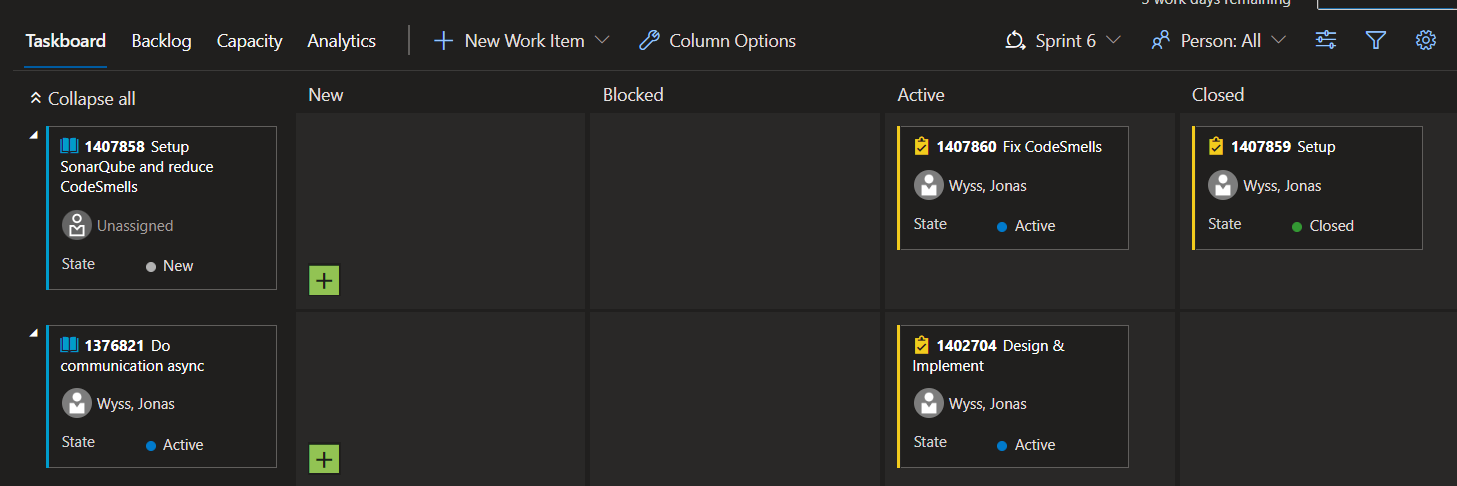
\includegraphics[width=1.0\textwidth]{gfx/ado.png}
   \caption{
         Ausschnitt aus dem Backlog des sechsten Sprints in \ac{ADO}
      }
      \label{fig:adosprint6}
\end{figure}
Wärend der Sprints soll das aktuelle Backlog jeweils einen Überblick über den aktuellen Stand der Arbeiten geben.
In Abbildung \ref{fig:adosprint6} ist gezeigt, wie dies ausschauen kann.

Zusätzlich sollen zwei weitere Funktionen von \ac{ADO} verwendet werden:
\begin{itemize}
   \item Der Quellcode soll in einem Repository abgelegt werden, welches von \ac{ADO} verwaltet wird.
   \item Die Pipelines von \ac{ADO} sollen für \ac{CICD} verwendet werden.
\end{itemize}

\section{Coding Standard}\label{codingStandard}
% TODO move to Konzepte?
Der C\# Code der für diese Arbeit geschrieben wird, befolgt den Coding Style der dotnet runtime \footnote{https://github.com/dotnet/runtime/blob/main/docs/coding-guidelines/coding-style.md}.
Die Entwicklungsumgebung Visual Studio ist standardmässig so konfiguriert, dass sie diesem Style folgt.
Sie unterstützt die Entwickler mit automatischen Formatierungen und weisst darauf hin, wenn der Standard verletzt wird. 

\section{Test Driven Development} \label{tdd}
\ac{TDD} ist ein Vorgehen zur parallelen Entwicklung von produktiv Code sowie Testfällen.
Dabei wird jeweils zuerst ein Testfall geschrieben, welcher fehlschlagen soll.
Danach wird genau so viel Code geschrieben, dass der Testfall abgedeckt ist.
Nun kann der geschrieben Code wenn nötig überarbeitet werden.
Bestehende Testfälle dürfen nicht gebrochen werden.
Diese Vorgehen wird solange wiederholt, bis alle benötigten Funktionen getestet und implementiert sind.
Ein Vorteil von \ac{TDD} ist, das Entwicklungsarbeit vorhersagbar wird.
Ist eine Funktion implementiert kann mit Sicherheit gesagt werden, dass diese auch richtig funktioniert \parencite{beck2003test}.

In dieser Arbeit sollen möglichst immer nach \ac{TDD} vorgegangen werden.


\section{Diagramme}
Diagramme welche während des Designprozesses erstellt werden, sollen mit PlantUML\footnote{https://plantuml.com/} erstellt und dem UML Standard folgen.
Dies gilt auch für jene Diagramme, die in dieser Arbeit aufgeführt werden.
\chapter{Realisierung}
% Dies ist das Hauptkapitel Ihrer Arbeit! Hier wird die Umsetzung der eigenen Ideen und Konzepte
% (Kapitel 3) anhand der gewählten Methoden (Kapitel 4) beschrieben, inkl. der dabei aufgetretenen
% Schwierigkeiten und Einschränkungen.
Die Realisierung lässt sich in drei Phasen unterteilen.

In der ersten Phase werden grundlegende Entscheidungen getroffen und die Basis der Arbeit implementiert.
Am Ende der ersten Phase existiert ein Prototyp,
welcher bei allen Komponenten des System die über minimale Funktionen verfügt. (TODO verweis )

Wie im Kapitel Vorgehen beschrieben (TODO), folgen darauf zwei weitere Phasen,
in welche neue Anforderungen des Auftraggebers umgesetzt werden.

\section{Grundlegende Designentscheidungen}

Der folgende Abschnitt gibt einen Überblick der gewählten Technologien und
der grundlegenden Designentscheidungen und wieso diese so umgesetzt wurden.

\subsection{Auswahl des Technologiestacks}

Bei er Auswahl des Technologiestacks wurde auf verschiedene Aspekte geachtet.
Zum einen sollte das Frontend unabhängig vom Backend entwickelt werden können.
Aus diesem Grund wurde für die Kommunikation, wie in Kapitel \ref{konzepte:api-kommunikation}
bereits beschrieben, eine \ac{REST} \ac{API} verwendet.
Auf die genaue Definition der \ac{API} wird in den nächsten Abschnitten noch genauer eingegangen.

Für die Implementation des Backends gibt es unzählige Technologien die man für eine \ac{CRUD}
Applikation verwenden kann (Siehe Kapitel \ref{state:backend}). Für dieses Projekt sollte
eine \ac{REST} \ac{API} implementiert werden können. Und die Datenbank soll über ein \ac{ORM}
abstrahiert werden können. Dies hat den Vorteil, dass die eigentliche Datenbanktechnologie
keine grosse Rolle spielt. Das \ac{ORM} abstrahiert die Tabellenstruktur mittels
Objekten im Sourcecode. Als Backend kann beispielsweise zum Testen und Entwickeln
eine Sqlite\footnote{https://www.sqlite.org/index.html} Datenbank verwendet werden.
Der gleiche Sourcecode kann danach in der Produktion auf eine PostgreSQL\footnote{https://www.postgresql.org/}
Datenbank zugreifen um besser zu skallieren.
Natürlich soll auch ein \ac{MQTT} Framework in der gewählten Technologie zur verfügung stehen
damit die Messdaten der Stromzähler empfangen und in die Datenbank abgespeichert werden können.

Python bietet für jedes dieser Anforderungen gleich mehrere Frameworks an. Mit Python können sehr
schnell Prototypen erstellt werden. Es eignet sich aber auch für grosse Produktivsoftware.
Einige der wohl Bekanntesten Programme wie YouTube, Instagram, Spotify oder Reddit sind
in Python geschrieben. \cite{popular_python_sw}

Bei der Implementation des Frontends wurde wie in Kapitel \ref{state:frontend} beschrieben
anhand der State of Js Umfragen React\footnote{https://reactjs.org/} verwendet.
Um nicht das ganze Benutzerinterface selber gestalten zu müssen, wurde eine Material Design\footnote{https://material.io/design}
Library verwendet.

Um die Applikation für die Entwicklung lokal aufzusetzen, zu testen oder zu Deployen wurde dazu
Podman verwendet (Siehe Kapitel \ref{state:deployment}).

\subsection{Datenbankschema}

Gleich zu beginn des Projektes wurde das Datenbankschema erstellt.
Dies gibt eine gute Übersicht ob die für das Projekt benötigten Daten
abgespeicher werden können. In diesem Fall sind das die Messwerte der Stromzähler
und die Labels des Benutzers.

Die Datenbank wurde so einfach wie möglich gehalten um alle vorgegebenen
Anforderungen zu erfüllen.

\begin{figure}[h]
    \centering
    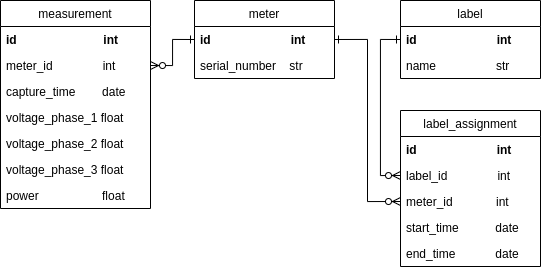
\includegraphics[width=1.0\textwidth]{gfx/smic-db}
    \caption{
        ER Diagramm der Datenbank
    }
    \label{fig:smic-db}
\end{figure}

Wie in Abbildung \ref{fig:smic-db} dargestellt, können in der Datenbank
die Verschiedenen Stromzähler mit ihrer Seriennumer abgespeichert werden.
Beispielsweise wird pro Haushalt ein Stromzähler mit einer bestimmten
Seriennummer abgespeichert, sobald dieser zum ersten mal Daten sendet.
Ein solcher Stromzähler sendet danach einzelne Messdaten zu bestimmten
Zeitpunkten. Die Messdaten beinhalten neben der Messzeit die drei Phasen
und wie viel Leistung gebraucht wurde.

Damit danach abgespeichert werden kann zu welcher Zeit beispielsweise ein
Toaster gelaufen ist, werden Labels erstellt. Ein solches Label hat eine
Bezeichnung und kann verschiedene Annotationen beinhalten.
Eine Annotation ist immer von einem bestimmten Stromzähler und kann implizit mehrere
Messdaten beinhalten. Dies wird über eine Start- und Endzeit abgespeichert.
Durch diese Struktur können danach einfach Auswertungen der Labels über mehrere
Stromzähler und Messpunkte gemacht werden.

\subsection{Architekturentscheidung}
\label{architekturentscheidung}

In dieser Arbeit wird keine Microservice Architektur im klassischen Sinne verwendet. (Siehe Kapitel \ref{konzepte:microservices})
Die einzelnen Komponenten werden zwar in separaten Container deployt (Abbildung: \ref{fig:smic-arch})
besitzen jedoch keine eigene Datenbank.
Das hat den Vorteil, dass weniger Overhead implementiert werden muss (mittels Message Queue)
und das Datenbankschema kann zentral in der Datastore Library einmal definiert
und dann in den verschiedenen Komponenten wiederverwendet werden.


\begin{figure}[h]
    \centering
    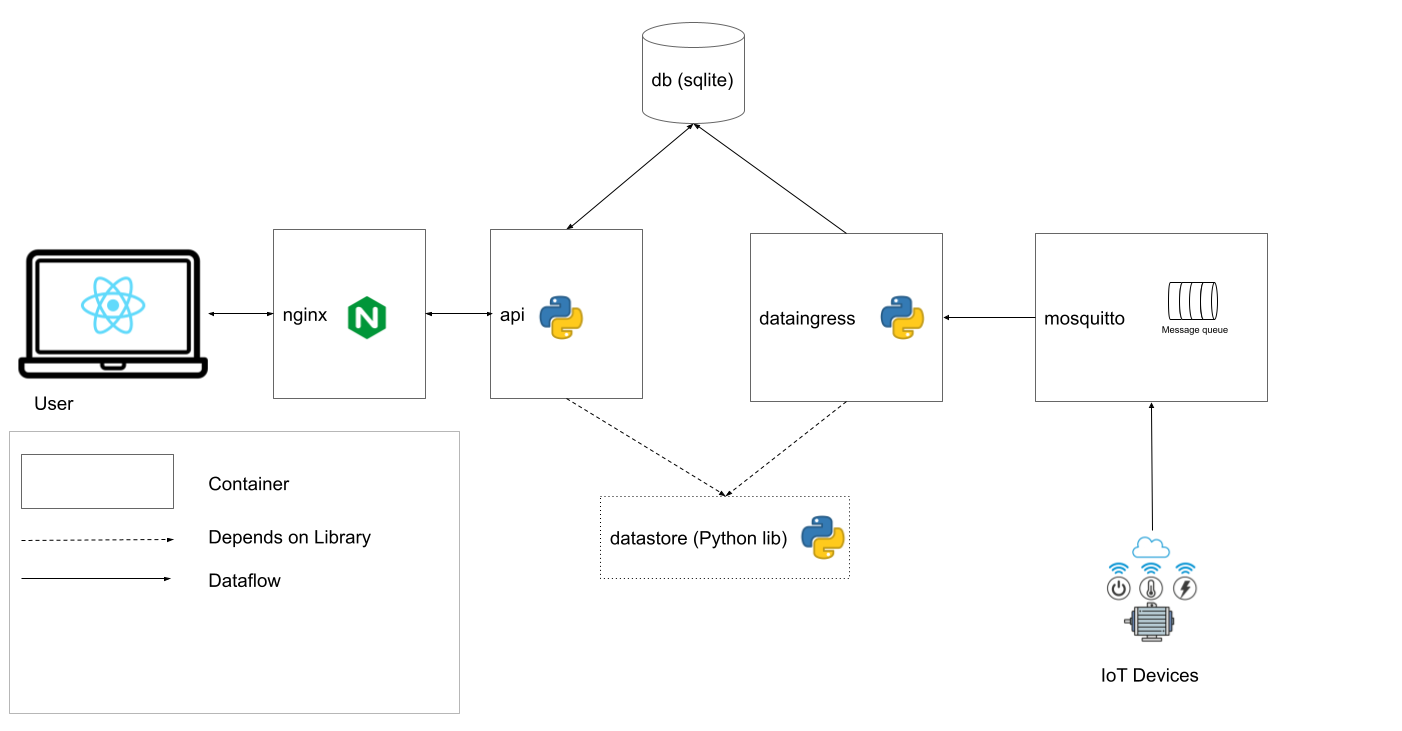
\includegraphics[width=1.0\textwidth]{gfx/smic-arch}
    \caption{
        Schematische Darstellung der in diesem Projekt verwendeten Architektur
    }
    \label{fig:smic-arch}
\end{figure}

Die Abbildung \ref{fig:smic-arch} zeigt die in diesem Projekt verwendete
Architektur auf. Hier noch einige Informationen zu den einzelnen Komponenten:


\begin{itemize}
    \item \texttt{nginx}:
        Alle Anfragen des Endbenutzers werden über einen Nginx Server
        entgegengenommen. Dieser liefert dann dem Benutzer die React WebApp
        oder leitet Anfragen an die \ac{API} weiter.

    \item \texttt{api}:
        Die \ac{API} verarbeitet Datenanfragen der React WebApp. Sie gibt
        beispielsweise die Stromzählerdaten eines Tages zurück.

    \item \texttt{datastore}:
        Der datastore ist eine Python library, die das Datenbankschema mittels \ac{ORM} festlegt.
        Sowohl die \ac{API} als auch der dataingress greifen auf die Datenbank zu
        und verwenden somit die datastore library.

    \item \texttt{dataingress}:
        Der dataingress arbeitet die von den \ac{IoT} Geräten gesendeten
        Stromzählerdaten ab und speichert diese in die Datenbank.

    \item \texttt{mosquitto}:
        Mosquitto ist der in dieser Arbeit verwendete \ac{MQTT} Broker.
\end{itemize}

Ein weiterer grund für die Entscheidung einer geteilten Datenbank ist,
dass der \texttt{dataingress} keine Daten liest, sondern diese nur von
der \ac{MQTT} Queue abarbeitet und in die Datenbank schreibt.

Auf die einzelnen Komponenten wird später in der Realisierungsphase noch genauer
eingegangen.

\subsection{Continous Integration, Contionous Delivery}

Um das Projekt automatisch Testen zu können und eine Reproduzierbare Umgebung zu bauen,
wurde bereits zu Beginn eine \ac{CI/CD} Pipeline mit GitHub Actions\footnote{https://github.com/features/actions}
aufgebaut.
Die Entwickler sollen sich nicht nur um die Entwicklung, sondern auch das automatische Bauen und Deployen der
Software kümmern. Dieser DevOps Gedanke hat den Vorteil, dass
theoretisch jedes kleine Feature und jeder Bugfix direkt automatisiert getestet
wird und danach (wenn die Tests erfolgreich waren) auf das Produktivsystem
Deployt werden kann. \cite{what_is_devops}
zudem ist für jeden Entwickler das Bauen und Ausführen des Projektes gleich und
reproduzierbar. Dies erspart das Suchen von unnötigen Fehlern die auf unterschiedlich
konfigurierten Entwicklungsmaschinen auftreten können.

\begin{figure}[h]
    \centering
    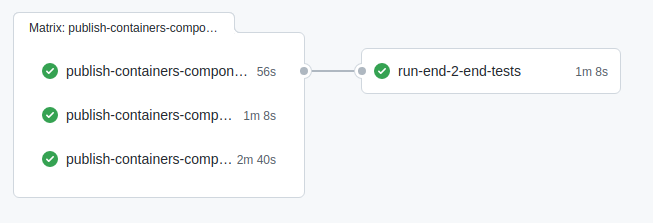
\includegraphics[width=1.0\textwidth]{gfx/ci-env}
    \caption{
        Visualisierung der GitHub Actions Pipeline mit zwei aufeinanderfolgenden Stages.
        Zuerst werden die einzelnen Komponenten (Siehe \ref{fig:smic-arch}) gebaut und
        anschliessend getestet.
    }
    \label{fig:ci-env}
\end{figure}

Dank dieser \ac{CI/CD} Umgebung und der Verwendung von Podman, kann die gesamte Applikation
(Wie im Kapitel \ref{architekturentscheidung} beschrieben) mit einem
Befehl gebaut und gestartet werden.

\section{Verarbeitung und Visualisierung von Stromzählerdaten}

In einer ersten Phase werden laut der Aufgabenstellung \ref{aufgabenstellung} Stromzähler
Messdaten per \ac{MQTT} empfangen und in eine Datenbank gespeichert.
Diese gespeicherten Daten werden dann in einer WebApp visualisiert und dem Benutzer
angezeigt.

\begin{figure}[h]
    \centering
    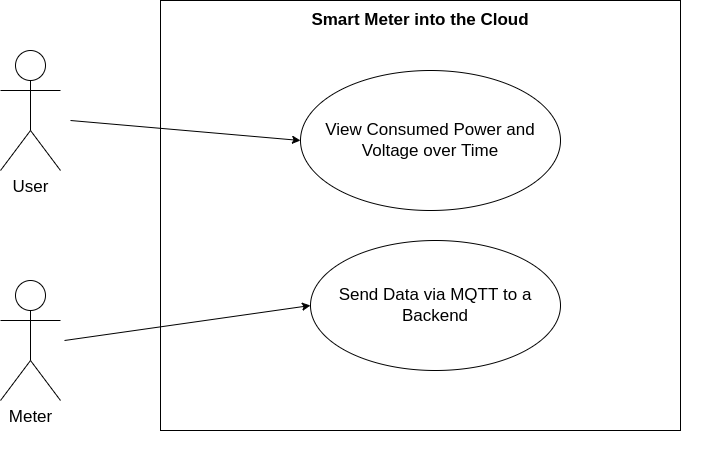
\includegraphics[width=1.0\textwidth]{gfx/usecase1}
    \caption{
        UseCase Diagramm der Verarbeitung und Visualisierung von Stromzählerdaten.
    }
    \label{fig:usecase1}
\end{figure}

\subsection{Frontend und Backend Abstraktion}

Damit die Arbeit von Frontend und Backend aufgeteilt werden kann, wurde zuerst
die \ac{API} Schnittstelle definiert. Für die Implementierung im Backend
stand die Entscheidung zwischen Flask\footnote{https://flask.palletsprojects.com/en/2.0.x/}
und FastAPI\footnote{https://fastapi.tiangolo.com/}.
Flask ist ein simples Web Framework mit dem \ac{API}s aber auch Server Side Rendering \cite{flask_server_side}
gemacht werden kann. FastAPI ist ein typisiertes Framework das darauf spezialisiert ist
\ac{REST} \ac{API}s zu implementieren. FastAPI ist ähnlich aufgebaut wie Flask aber auf den
\ac{API} Bereich spezialisiert. Die Dokumentation wird auch automatisch generiert.
FastAPI eignet sich perfekt um die \ac{API} zwischen Frontend und Backend zu implementieren.

\begin{figure}[h]
    \centering
    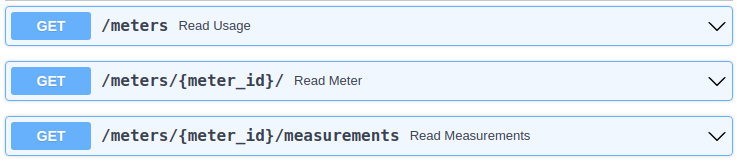
\includegraphics[width=1.0\textwidth]{gfx/api-visualization}
    \caption{
        \ac{API} Definition für die Visualisierung von Stromzählerdaten
    }
    \label{fig:api-visualization}
\end{figure}

Wie in Abbildung \ref{fig:api-visualization} dargestellt, besteht die \ac{API} der Stromzähler
und Messdaten ausschliesslich aus Abfragen. Die zu speichernden Daten kommen dann (wie im nächsten
Abschnitt erklärt) aus den \ac{MQTT} Daten der Stromzähler selbst.

\begin{figure}[h]
    \centering
    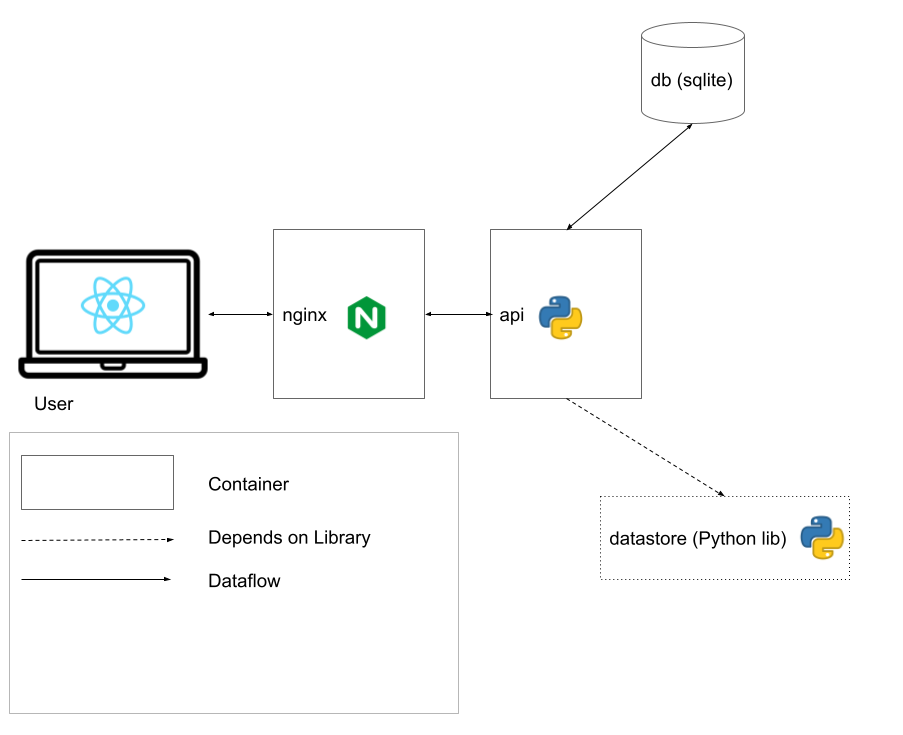
\includegraphics[width=0.8\textwidth]{gfx/sim-arch-api}
    \caption{
        Architektur der \ac{API} zwischen Frontend und Backend
    }
    \label{fig:arch-visualization-front-back}
\end{figure}

Sobald die WebApp von einem Benutzer aufgerufen wird, lifert der Nginx Server
die WebApp per \ac{HTTP} request aus. (Abbildung \ref{fig:arch-visualization-front-back})
Wenn der Benutzer (in diesem Fall über das React Web Frontend) danach die Messdaten seines
Stromzählers abfragen will, wird ebenfalls eine Asynchrone \ac{HTTP} Anfrage an die Backend \ac{API} gemacht.
Die Abfrage landet dann beim Nginx und wird an das Python FastAPI Backend weitergeleitet.
Dieses Python Backend führt danach eine SQL Abfrage via \ac{ORM} auf der Datenbank aus.
Um die Daten im Web Frontend anzeigen zu können, werden sie noch \ac{JSON} serialisiert
und zurück an die WebApp gesendet.

Die datastore Python Library stellt der \ac{API} das Datenbankschema zur Verfügung,
damit das \ac{ORM} die Abfragen an die Datenbank machen kann.
Als \ac{ORM} Framework wird sqlmodel\footnote{https://github.com/tiangolo/sqlmodel} verwendet.
Sqlmodel wird vom gleichen Entwickler wie FastAPI maintaint und bietet eine gute Integration.

Da nun das Datenmodell (in der datastore Library) und die \ac{API} definiert wurden,
kann das Web Frontend unabhängig vom Verarbeiten der \ac{MQTT} Daten gemacht werden.

\subsection{Implementation der Backend \ac{API}}

Wie alle Python Komponenten dieses Projektes wird auch das Backend \ac{API}
als Python Poetry\footnote{https://python-poetry.org/} Projekt implementiert.
Poetry verbessert das Paketmanagement von Python erheblich gegenüber Setuptools
und pip. \cite{python_poetry}
Dadurch ist es auch einfacher die Applikation als Container zu bauen und
damit einen reproduzierbaren Build zu garantieren.

Die Datenbankanbindung kann per Datenbank \ac{URI} dem sqlmodel Framework
mitgegeben um zu bestimmen auf welche Datenbank zugegriffen werden soll.

\subsection{Implementation der Datenvisualisierung}

TODO: Jonas

\subsection{\ac{MQTT} Datenverarbeitung}

Die Daten der Stromzähler werden per \ac{MQTT} an den Broker gesendet. \ref{state:mqtt}

\begin{figure}[h]
    \centering
    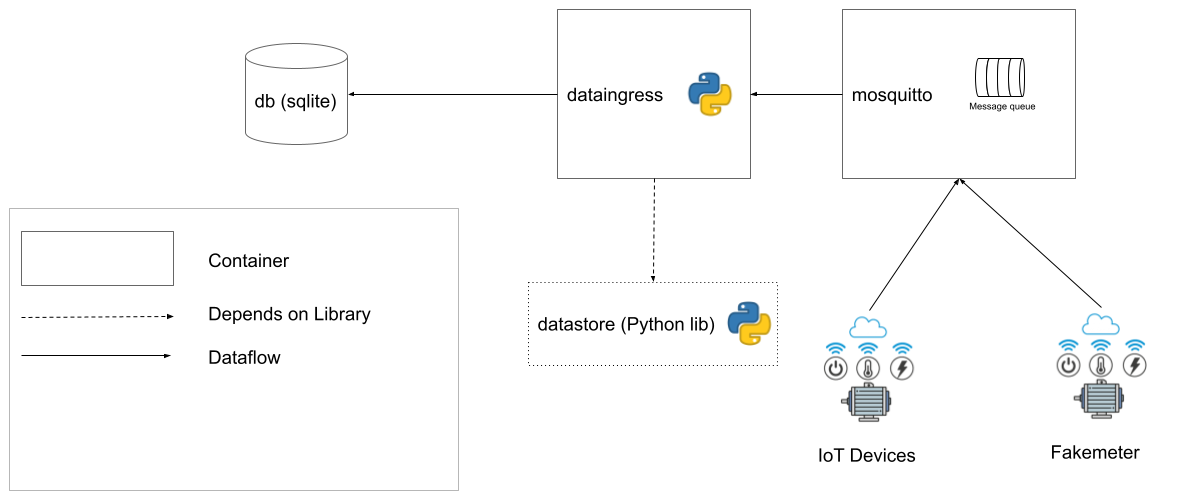
\includegraphics[width=1.0\textwidth]{gfx/smic-arch-mqtt}
    \caption{
        Architektur des \ac{MQTT} Messagebroker und des Dataingress welcher die
        empfangenen Nachrichten in die Datenbank persistiert.
    }
    \label{fig:arch-mqtt}
\end{figure}

Der Dataingress (ebenfalls ein Python Poetry projekt) registriert sich dann auf die von
den Stromzählern gesendeten Events und arbeitet diese ab. Das Empfangen und Abarbeiten, bzw.
in die Datenbank schreiben wird von unterschiedlichen internen Komponenten übernommen.
Beim Abarbeiten wird zudem, falls ein Datensatz nicht prozessiert werden kann dies noch
einmal versucht. Beispielsweise kann die Datenbank noch nicht bereit sein.\footnote{
    Das kann beispielsweise passieren, wenn die Datenbank neu gestartet wird nach einem update.
}
Dadurch soll möglichst verhindert werden, dass eingehende Messdaten verloren gehen.

\begin{figure}[h]
    \centering
    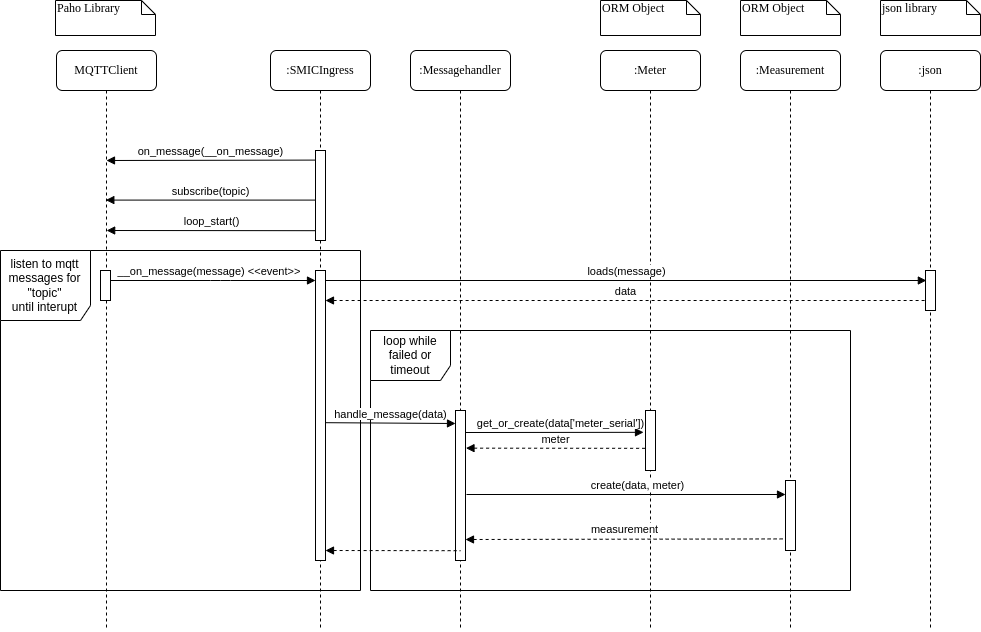
\includegraphics[width=1.0\textwidth]{gfx/dataingress-sequence}
    \caption{
        Das Sequenzdiagramm zeigt auf wie der Dataingress die \ac{MQTT} Messages
        von den Stromzählern abarbeitet und in die Datenbank persisitiert.
    }
    \label{fig:dataingress-sequence}
\end{figure}

\section{Demo nach der ersten Phase}
Screenshot der ersten version
Rückmeldungen:
- grundsätzlich zufrieden
- Mobile nicht weiter zentral, Fokus auf Dashboard, Desktop

Neue Anforderungen:
Range/Zähler auswählen sowie typ der Daten
echte Daten automatisiert einspielen
THD und Power zusätzlich zu Spannung

\section{Demon nach der zweiten Phase}
- Labeling:
Labels graphisch darstellen
Labels mittels UI hinzufügen

\chapter{Evaluation und Validation}
% Reflexion der eigenen Arbeit, ungelöste Probleme, weitere Ideen.

\chapter{Ausblick}

\section{ATS aufsplitten}\label{ausblick:ats_split}
Einzelnen Komponenten wie bswp. DLMS kommunikation als NuGet Paket bereitstellen.


\section{Class Descriptions}
Wie werden dies aktuell gehalten?


\subsection{Testagent mit Zähler}
Im Abschnitt \ref{Integrationstests} wurde beschrieben, dass für das ausführen der Integrationstests ein angeschlossener Stromzähler vorausgesetzt wird.
TODO

\subsection{SonarQube}
In Abschnitt \ref{s6:sonar} wurde erklärt, wieso im Rahmen dieser Arbeit lediglich eine lokale Instanz des Qualitätssicherungstools SonarQube eingesetzt wurde.
Für den Unterhalt und die Weiterentwicklung der Anwendung sollte jedoch eine Instanz auf einem Server eingesetzt werden, welche mit dem \ac{CI} Server verbunden ist.
Dies hätte zwei Vorteile:
\begin{itemize}
   \item Die Berichte zu Codequalität werden bei jeder Änderung des Codes automatisch erstellt. 
Entwickler müssen sich nicht selber darum kümmern.
   \item Die Metriken zur Qualität der Anwendung sind für alle Personen einsehbar.
\end{itemize}
%*************************************************************************
% Recommendations
%*************************************************************************
%\part{Empfehlungen zur Erstellung wissenschaftlicher Abschlussarbeiten}
%\label{pt:recommendations}
%*************************************************************************
% Backmatter
%*************************************************************************
% \appendix
%\renewcommand{\thechapter}{\alph{chapter}}
\cleardoublepage
% \part{Appendix}
\chapter{Aufgabenstellung.pdf}
\label{anhang:aufgabenstellung}
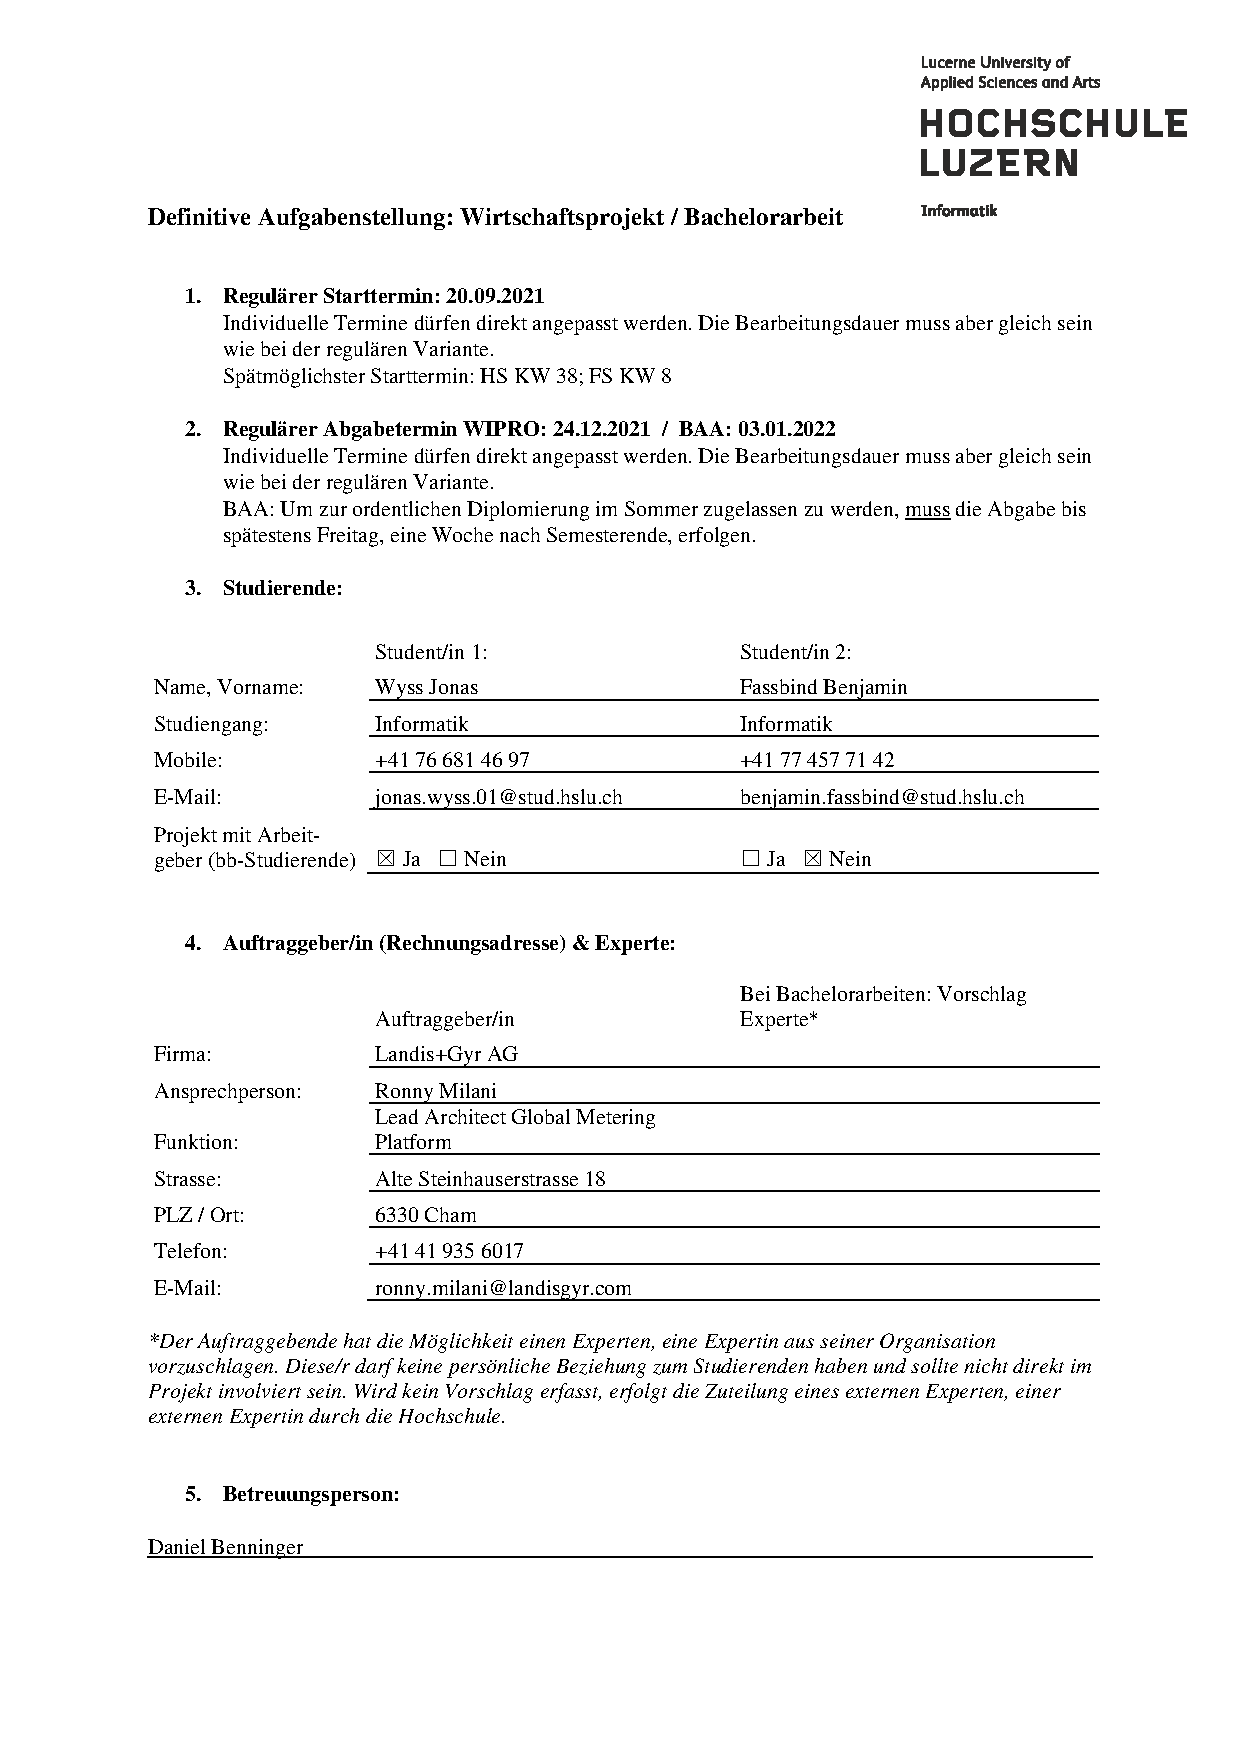
\includepdf[pages=-]{anhang/Aufgabenstellung.pdf}


\chapter{DMT2\_Quick\_Access\_survey.pdf}
\label{anhang:survey}
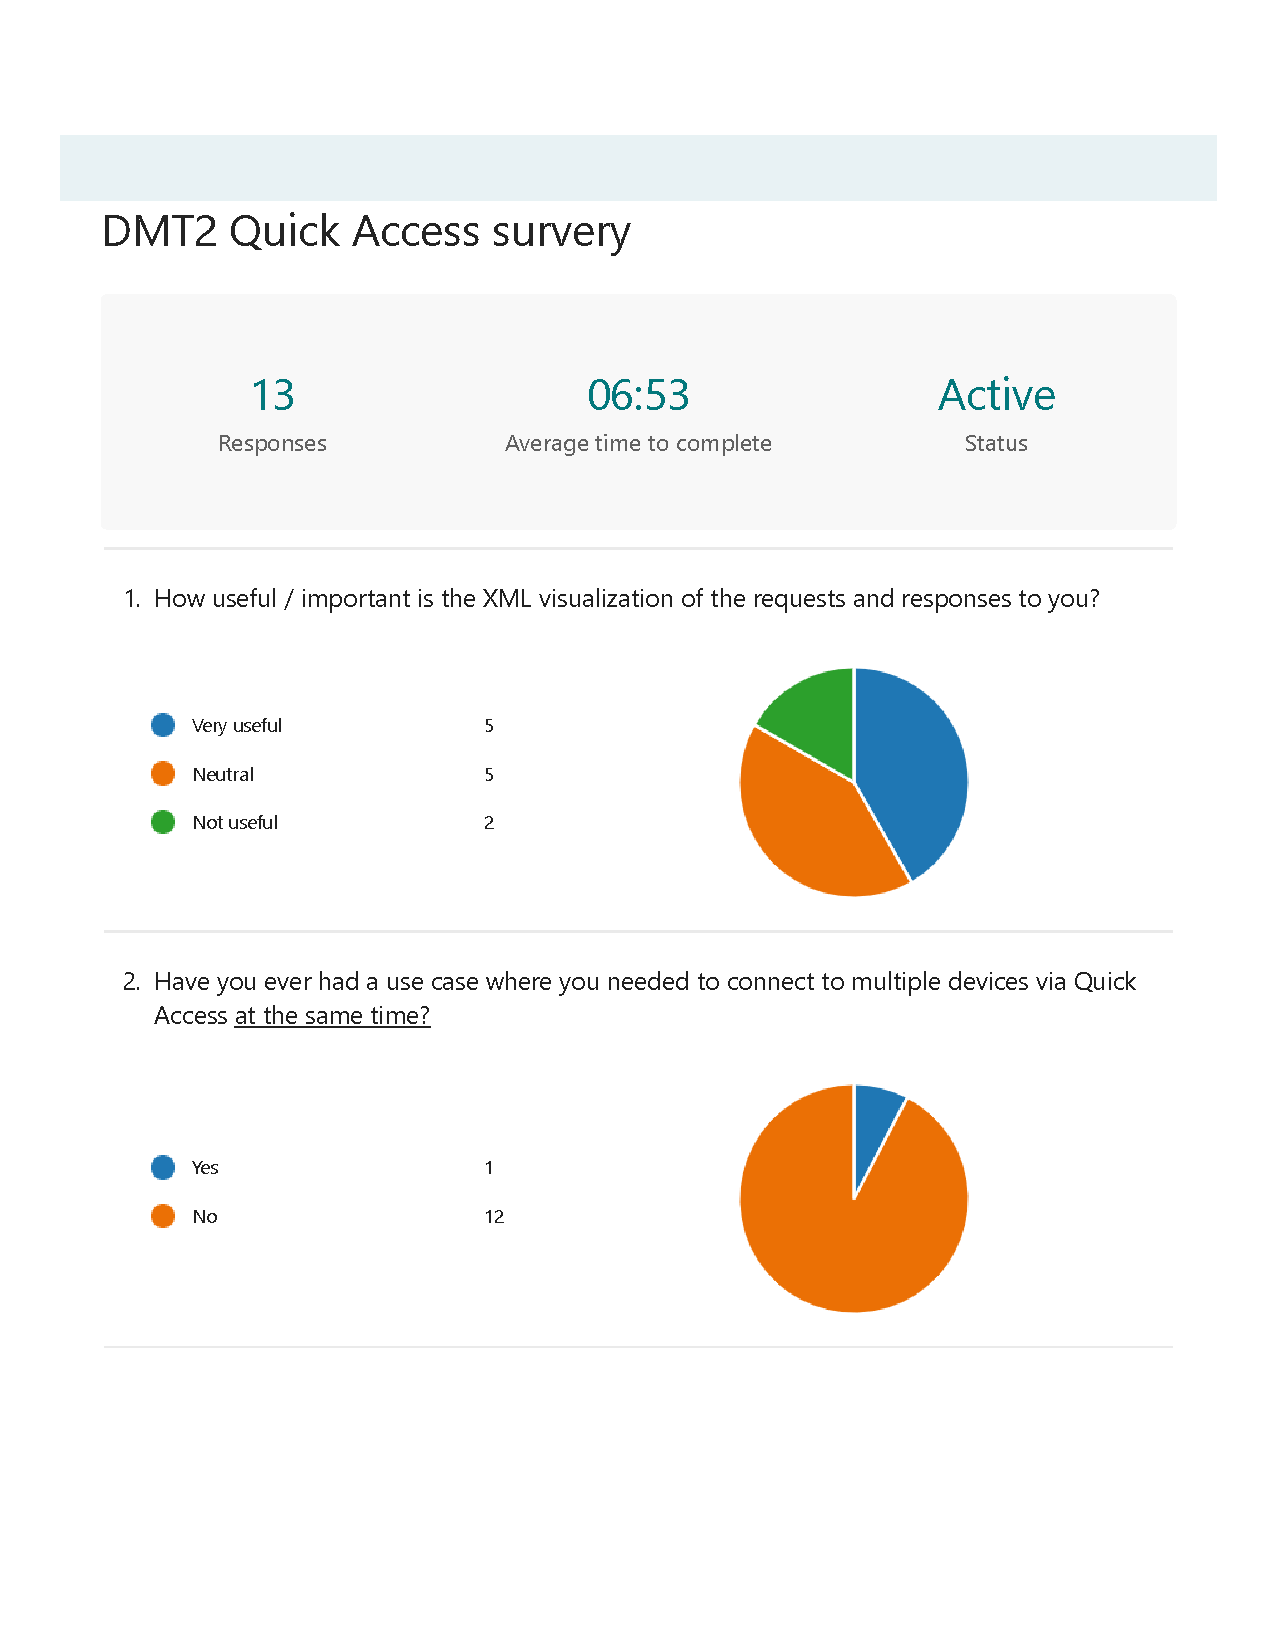
\includepdf[pages=-]{anhang/DMT2_Quick_Access_survey.pdf}
\cleardoublepage%*******************************************************
% List of Figures
%******************************************************* 
\automark[section]{chapter}
\renewcommand{\chaptermark}[1]{\markboth{\spacedlowsmallcaps{#1}}{\spacedlowsmallcaps{#1}}}
\renewcommand{\sectionmark}[1]{\markright{\thesection\enspace\spacedlowsmallcaps{#1}}}
\refstepcounter{dummy}
\pdfbookmark[0]{\listfigurename}{lof}
\listoffigures

\cleardoublepage

\cleardoublepage%*******************************************************
% Acronyms
%*******************************************************
\automark[section]{chapter}
\renewcommand{\chaptermark}[1]{\markboth{\spacedlowsmallcaps{#1}}{\spacedlowsmallcaps{#1}}}
\renewcommand{\sectionmark}[1]{\markright{\thesection\enspace\spacedlowsmallcaps{#1}}}
\refstepcounter{dummy}
\pdfbookmark[0]{Abk\"{u}rzungsverzeichnis}{abkuerzungsverzeichnis}
\markboth{\spacedlowsmallcaps{Abk\"{u}rzungsverzeichnis}}{\spacedlowsmallcaps{Abk\"{u}rzungsverzeichnis}}
\chapter*{Abk\"{u}rzungsverzeichnis}

% Insert your acronyms here
\begin{acronym}[UML]
  \acro{DRY}{Don't Repeat Yourself}
  \acro{ADO}{Azure DevOps}
  \acro{DLMS}{Device Language Message Specification}
  \acro{COSEM}{Companion Specification for Energy Metering}
  \acro{ATS}{Automated Test System}
  \acro{IEEE} {TODO}
  \acro{OSI} {Open System Interconnection}
  \acro{OBIS} {Object Identification System}
  \acro{CLI} {Command Line Interface}
  \acro{WPF} {Windows Presentation Foundation}
  \acro{MVVM} {Model-View-ViewModel}
  \acro{CI} {Continuous Integration}
  \acro{SCM} {Source Code Management}
  \acro{DMT2} {Dlms Multi Tester 2}
  \acro{TDD} {Test Driven Development}
  \acro{CICD} {Continuous Integration, Continuous Delivery}
  \acro{TLS} {Transport Layer Security}
  \acro{YAML} {YAML Ain't Markup Language}
  \acro{UWP} {Universal Windows Platform}

\end{acronym}

\cleardoublepage

%*************************************************************************
% Other Stuff in the Back
%*************************************************************************
\cleardoublepage%********************************************************************
% Bibliography
%*******************************************************
% work-around to have small caps also here in the headline
% https://tex.stackexchange.com/questions/188126/wrong-header-in-bibliography-classicthesis
% Thanks to Enrico Gregorio
\defbibheading{bibintoc}[\bibname]{%
  \phantomsection
  \manualmark
  \markboth{\spacedlowsmallcaps{#1}}{\spacedlowsmallcaps{#1}}%
  \addtocontents{toc}{\protect\vspace{\beforebibskip}}%
  \addcontentsline{toc}{chapter}{\tocEntry{#1}}%
  \chapter*{#1}%
}
\printbibliography[heading=bibintoc]

%*************************************************************************
% Game Over: Restore, Restart, or Quit?
%*************************************************************************
\end{document}
%*************************************************************************

